\documentclass[manuscript, screen, review, acmsmall, anonymous]{acmart}
%\documentclass[acmsmall,authorversion]{acmart}
\usepackage{subcaption}
\usepackage{hyperref}

\newcommand{\TODO}[1]{\textcolor{red}{#1}}

\usepackage[skins, breakable]{tcolorbox}
%% \BibTeX command to typeset BibTeX logo in the docs
\AtBeginDocument{%
  \providecommand\BibTeX{{%
    Bib\TeX}}}

\begin{document}

\title{Generative AI and Creativity: A Systematic Literature Review and Meta Analysis}

\author{Niklas Holzner}
\email{n.holzner@campus.lmu.de}
\affiliation{
  \institution{LMU Munich}
  \city{Munich}
  \state{Bavaria}
  \country{Germany}
}
\author{Sebastian Maier}
\email{maier.sebastian@campus.lmu.de}
\affiliation{
  \institution{LMU Munich \& Munich Center for Machine Learning (MCML)}
  \city{Munich}
  \state{Bavaria}
  \country{Germany}
}
\author{Stefan Feuerriegel}
\email{feuerriegel@lmu.de}
\affiliation{
  \institution{LMU Munich \& Munich Center for Machine Learning (MCML)}
  \city{Munich}
  \state{Bavaria}
  \country{Germany}
}
\begin{abstract}
Generative artificial intelligence (GenAI) is increasingly used to support a wide range of human tasks, yet empirical evidence on its effect on creativity remains scattered. Can GenAI generate ideas that are creative? To what extent can it support humans in generating ideas that are both creative and diverse? In this study, we conduct a meta-analysis to evaluate the effect of GenAI on the performance in creative tasks. For this, we first perform a systematic literature search, based on which we identify $N$ = XX relevant studies for inclusion in our meta-analysis. We then compute standardized effect sizes based on Hedges' $g$. We compare different outcomes: (i)~how creative GenAI is; (ii)~how creative humans augmented by GenAI are; and (iii)~the diversity of ideas by humans augmented by GenAI. Our results indicate a small, statistically non-significant improvement in human creative performance ($g$ = X.XX), and a comparable but statistically significant creative performance for humans supported by GenAI ($g$ = X.XX). Further, GenAI has a positive effect on the diversity of ideas for such collaborations between humans and GenAI ($g$ = X.XX). We further analyze heterogeneity across different types of GenAI models (e.g., text-to-text, text-to-image), different tasks (e.g., creative writing, ideation), different measurements (e.g., novelty, originality), and different participant populations (e.g., laypeople vs. domain experts). Overall, our results position GenAI as an augmentative tool that can support, rather than replace, human creativity---particularly in tasks benefiting from ideation support.
\end{abstract}

\maketitle
\section{Introduction}
\label{sec:Introduction}

% Gen AI

Generative artificial intelligence (GenAI) refers to a class of machine learning technologies that have the capability to generate new content that resembles human-created output, such as images, text, audio, and videos  \cite{FeuerriegelBISE2024}. GenAI can thus support various human tasks such as writing, software development, composing lyrics, and academic research, often at a performance similar to that of humans \TODO{add: https://journals.aom.org/doi/10.5465/amj.2023.4006}\cite{Herbold2023, Cui2025, 10.1093/pnasnexus/pgae052, Ruksakulpiwat2024, brynjolfsson2024generativeaiwork}. On top of that, Generative AI has also become a valuable tool in creative industries---spanning graphic design, advertising, fashion, writing, and visual arts  \TODO{Eine Ref von Jochen Hartmann/TUM
plsu: https://pubsonline.informs.org/doi/10.1287/mksc.2023.0494}\cite{Sun_2024}. 

Yet, empirical evidence on the benefits of GenAI for creative performance is scattered, and the theoretical arguments are often inconsistent or even contradictory. On the one side, cognitive research argues that creativity is an inherently human trait \cite{aru2024artificialintelligenceinternalprocesses,sæbø2024stochasticshumanartificialcreativity}. One common issue in practice is that GenAI models often lack the tacit knowledge required for systematic, compositional reasoning such as multi‐step problem solving to generate ideas perceived as creative, especially in real-world tasks from businesses. Similarly, GenAI is likely to reproduce ideas seen during training rather than ideating novel ideas \cite{ismayilzada2024creativityaiprogresseschallenges}. Hence, simply by means of the training data of GenAI, the generated ideas may also be less diverse than those of humans \cite{doi:10.1126/sciadv.adn5290}. On the other side, there is early evidence suggesting that outputs from GenAI are perceived as being creative \cite{wang2024aicreativehumans}. For example, several studies find benefits from GenAI in creative tasks, but these findings are typically limited to specific creative tasks (e.g., story writing, ideating business models) \cite{doi:10.1126/sciadv.adn5290, Lee2024, Zhou2024, Wadinambiarachchi_2024}. This may suggest that GenAI can generally improve creativity but it is often unclear how well the results generalize across domains.  

Here, we perform a meta-analysis to evaluate the effect of GenAI on creative performance.\footnote{Code and data for review are available via \TODO{Anonymized Git}. Upon acceptance, we will move both code and data to a public GitHub repository.} For this, we focus on different outcomes, namely: (i)~how creative GenAI is; (ii)~how creative humans augmented by GenAI are; and (iii)~the diversity of ideas by humans augmented by AI.\footnote{We also considered a fourth outcome, namely, the diversity of ideas generated by humans with GenAI support. Yet, our literature search did not return a sufficient number of empirical studies for this outcome. Hence, we refrain from analyzing this outcome. However, we identify this gap as a promising opportunity for future research, which we elaborate on in the discussion section.} To this end, we analyze the following \textbf{research questions (RQs)}:

\begin{itemize}
\item \textbf{RQ1:} \textit{How creative are ideas generated by GenAI (compared to humans without GenAI support)?}
\item \textbf{RQ2a:} \textit{How creative are ideas generated by humans when supported by GenAI (compared to humans without GenAI support)?}
\item \textbf{RQ2b:} \textit{How diverse are ideas generated by humans when supported by GenAI (compared to humans without GenAI support)?}
\end{itemize}

\noindent
To answer the above research questions, we first perform a systematic literature search and then conduct a meta-analysis. Overall, we retrieved $N= 693$ studies for inclusion, and eventually identified $N = TBA$ studies with empirical results. We then calculated the standardized effect size Hedges' $g$ and computed a random-effects meta-analysis. \TODO{hetoergeneity IMHO raus nehmen, nur potential bias (aber vlt kan under sastz auch ganz weg bzw. in wine klammer => ich ahbe ja am Ende den querverweis für anhang }We conduct several sensitivity analyses, meta-regressions, and Egger’s tests to address heterogeneity and potential bias. We further ran a moderator analysis on study heterogeneity across different GenAI model types (e.g., text-to-text, text-to-image), different tasks (e.g., creative writing, ideation), and different participant populations (e.g., laypeople vs. domain experts). to provide a general but differentiated understanding of the effect of GenAI on creativity. Additional robustness checks are reported in the \TODO{cross ref supplements}.

\begin{figure}
  \centering
  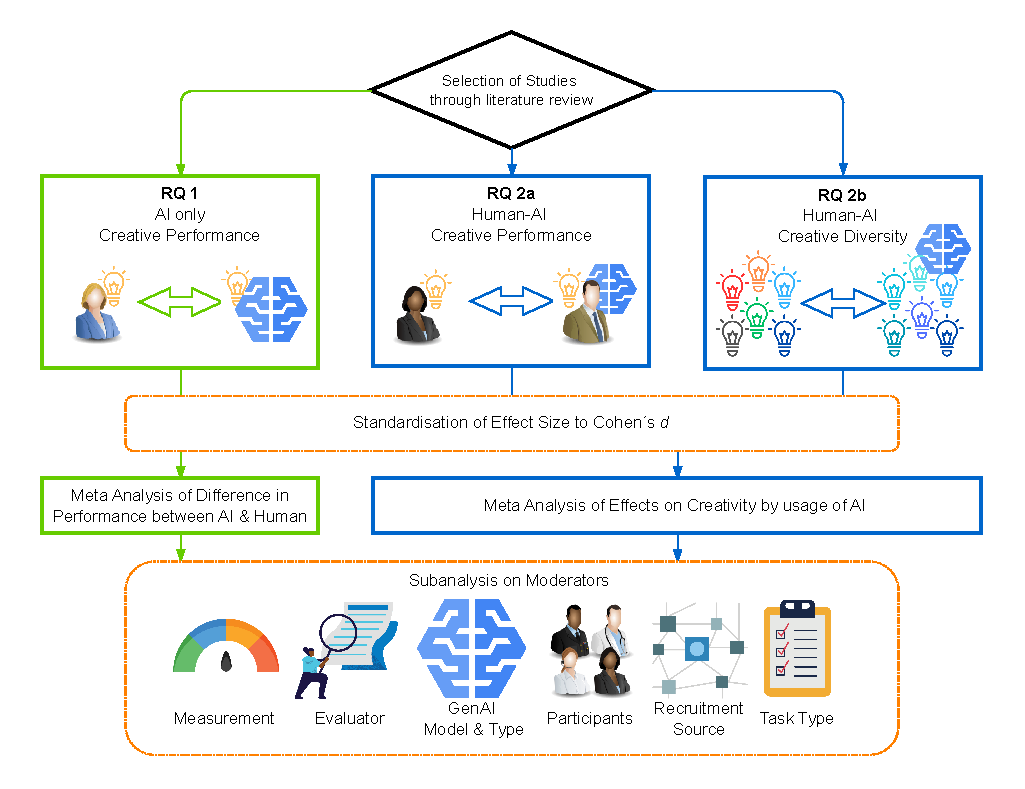
\includegraphics[width=0.9\linewidth]{overview.pdf}
  \caption{\textbf{Overview of the meta-analysis procedure.} We address three research questions: (RQ1) creative performance of GenAI alone, (RQ2a) creative performance of humans supported by GenAI, and (RQ2b) diversity of ideas in human–GenAI collaboration. After selecting studies via systematic literature review, we standardize effect sizes (Cohen’s $d$) and conduct meta-analyses, including a moderator analysis to study heterogeneity across types of GenAI models, tasks, measurements, and participant populations.}
\end{figure}


\section{Methods}
\label{sec:Methods}

In this section, we describe our data collection to identify relevant studies and statistical analysis. 

\subsection{Search Strategy}

Key definitions forming the basis for our understanding of creativity in the context of our meta analysis are \TODO{search included studies for creativity definitions}: 
\begin{figure}[h!]
    \label{fig:earch-query}
  \centering
  \begin{tcolorbox}[
    enhanced,
    breakable,
    center upper, 
    colback=gray!10,
    colframe=gray!60!black,
    boxrule=0.8pt,
    arc=4pt,
    outer arc=4pt,
    drop shadow={black!50!white,opacity=0.3},
    width=\textwidth,
    title=\textbf{Creativity}
  ]
    \begin{verbatim}
    novelty, originality, creativity
    \end{verbatim}
  \end{tcolorbox}
  \caption{Definition of creativity for our meta-analysis.}
  \label{fig:search-query}
\end{figure}
\begin{figure}[h!]
    \label{fig:earch-query}
  \centering
  \begin{tcolorbox}[
    enhanced,
    breakable,
    center upper, 
    colback=gray!10,
    colframe=gray!60!black,
    boxrule=0.8pt,
    arc=4pt,
    outer arc=4pt,
    drop shadow={black!50!white,opacity=0.3},
    width=\textwidth,
    title=\textbf{Creative diversity}
  ]
    \begin{verbatim}
    cosine similarity
    \end{verbatim}
  \end{tcolorbox}
  \caption{Definition of creative diversity for our meta-analysis.}
  \label{fig:search-query}
\end{figure}
    
    

To ensure transparency, reproducibility, and quality of our meta-analysis, we follow the PRISMA 2020 framework for systematic literature reviews \TODO{PRISMA 2020 Checklist} \TODO{citation PRISMA Checklist}. To identify relevant studies, we searched the following databases: (i)~Web of Science, (ii)~SSRN, and (iii)~arXiv. Our search includes non-peer-reviewed studies to reflect the rapidly evolving nature of GenAI research and to capture recent advances. Our search was limited to publications in the English language from the past five years, which is loosely aligned with the emergence of foundational models such as GPT and BERT. The knowledge cutt search was conducted on May 2, 2025.

Our search query is intentionally broad to include various ways to relate to GenAI technology and creativity. Overall, our search query is inspired by Schemmer et al.\,(2022) \cite{Schemmer2022} \TODO{citation Schemmer}, but which we adapted to our research question, namely, creativity:

  \begin{tcolorbox}[
    enhanced,
    breakable,
    center upper, 
    colback=gray!10,
    colframe=gray!60!black,
    boxrule=0.8pt,
    arc=4pt,
    outer arc=4pt,
    drop shadow={black!50!white,opacity=0.3},
    width=\textwidth,
    fontupper=\footnotesize,
    title=\textbf{Search query}
  ]
    \begin{verbatim}
    TITLE("creativity" OR "creative" OR "ideation" OR "idea")
    AND
    ("AI" OR "Artificial Intelligence" OR "LLM" OR "Large Language Models")
    \end{verbatim}
  \end{tcolorbox}


The process for inclusion/exclusion in our systematic literature review is shown in Figure~\ref{fig:PRIMSAFlowchart} (based on the format of the PRISMA 2020 Flowchart \TODO{citation PRISMA Flowchart}). Literature screening, eligibility checks, and final inclusion were performed by one person (the first author). In the identification phase, $N$ = 691 publications were identified by our search query, and out of which $n$ = 96 duplicate publications were removed manually. Out of the remaining $n$ = 595 publications, both the title and abstract were screened for inclusion in the assessment of eligibility. Here, \TODO{würde ich nicht unterscheiden (und auch im PRISMA bündeln) $n$ = 182 AND $n$ = 334} publications were excluded due to a lack of fit (e.g., a focus on legal studies). 

Subsequently,  $n$ = 79 records were assessed for eligibility. Studies were eligible if they:
\begin{enumerate}
  \item The study design was aimed at comparing (a)~the creativity performance of humans versus GenAI or (b)~the creative performance of humans with vs. without GenAI support. The study further followed a between-subject design, which is crucial to make rigorous statistical comparisons. 
  \item The study had to report sufficient statistics for computation of standardized effect size Hedges’ $g$. 
  \item Do not have the main topic of developing certain software or GenAI to prevent bias
  \item Do not provide raw data to prevent mistakes when handling unknown data
%  \item Are published in English
%  \item Are published within the last 5 years
%  \item Are peer-reviewed
%  \item Are openly accessible through our databases
\end{enumerate}
In this stage, records were excluded due to (i) insufficient study design ($n$ = 33) (ii) insufficient statistics ($n$ = 8) (iii) insufficient creativity measurement ($n$ = 4) (iv) insufficient data reporting ($n$ = 2). 

\subsection{Data Collection}

We contacted 15 authors via e-mail due to (ii) insufficient statistics or (iv) insufficient data reporting. If we have not received a reply on the first try, we followed up with a second e-mail to maximize the amount of included studies. From this we received additional sufficient information on ($n$ = 4) records for inclusion. All studies without reply were execluded under their original exclution criteria.


\begin{figure}[H]
  \centering
  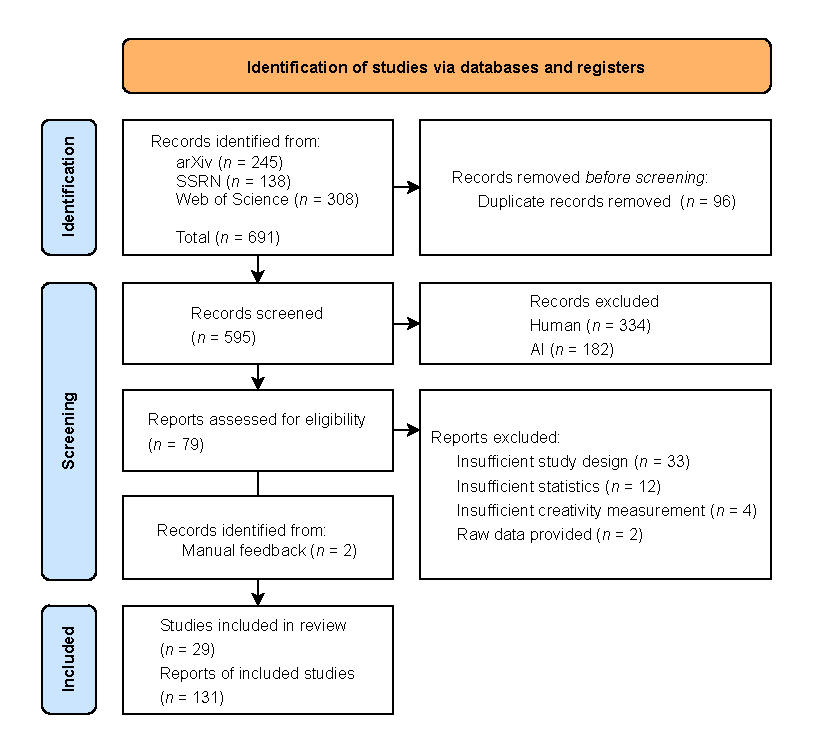
\includegraphics[width=\linewidth]{PRISMA_Flowchart}
  \caption{PRISMA Flow Chart.\TODO{finalize Montag (possible Feedback)}}
  \Description{PRISMA Flow Chart of the Literature Research.}
  \label{fig:PRIMSAFlowchart}
\end{figure}
We found $n$ = 27 studies to be eligible for our meta-analysis. Uncertainty in the screening or eligibility test procedure was resolved through discussion until consensus was reached with the advising experts \footnote{Author 2 and Author 3 acted as the independent working expert for consultation of Author 1 in the screening, eligibility procedure and statistical analysis.}.

Due to the novel scope of the research questions and the limited amount of eligible studies, we were aware that the search query could miss out on relevant studies. Therefore, author 2 and author 3 critically searched further databases for eligible studies. Two studies were identified by the experts and included (see Fig.~\ref{fig:PRIMSAFlowchart}). Thereby $n$ = 29 studies, that were compatible with each outcome domain, were included and manually recorded in our database by the first author. Extracted study‐level data of eligible records included study metadata (title, author, abstract, publication date, identification), experimental design details (task type, GenAI type, GenAI model, creativity measurement, measurement evaluator), participant characteristics (recruitment source, professional domain), and outcome statistics (means, $SD$, $SE$, $n-total$, $n-control$ and $n-treatment$, $F$-value, standardized $\beta$ and $SE-\beta$). If studies reported multiple measurements per experiment, expert measurements were preferred and included. If studies reported multiple experiments, each experiment was included with one measurement. \TODO{A comprehensive extraction sheet capturing all study features and outcomes is deposited in our project repository for transparency.} The coded moderators and their levels are summarized in Table ~\ref{tab:moderator_characteristics}. 

\begin{table}[H]
  \centering
  \label{tab:moderator_characteristics}
  \begin{tabular*}{\linewidth}{@{\extracolsep{\fill}} l | p{0.7\linewidth} }
    \toprule
    \textbf{Dimensions} & \textbf{Values} \\
    \midrule
    GenAI Type & text-to-text (T2T), text-to-image (T2I) \\
    \midrule
    GenAI Model & multiple models, GPT-4o, GPT-4, GPT-4all, GPT-3.5-turbo, GPT-3.5, GPT-3, Claude, SparkDesk, Qwen, Dou\,Bao, alpaca, bing, dolly, koala, oa, stablelm, vicuna, not disclosed (n.d.) \\
    \midrule
    Participants & Academia, Business, Science, lay people, not disclosed \\
    \midrule
    Recruitment Source & University, Prolific, Mturk, Public, Company \\
    \midrule
    Task Type & alternate uses task (AUT), consequences task (CT), divergent associations task (DAT), forward flow (FF), creative writing, creative problem solving, creative thinking, divergent thinking, ideation product, ideation item usage, ideation research proposal, ideation business concepts, ideation other\\
    \midrule
    Creativity Measurement & creativity scale, originality scale, novelty scale, semantic distance, cosine similarity, creative problem solving scale, flexibility score \\
     \midrule
    Measurement Evaluator & self-assessed, lay people, expert, rule-based, AI \\
    \addlinespace
    \bottomrule
  \end{tabular*}
  \caption{Descriptive characteristic values per moderator}
\end{table}

\subsection{Statistical Analysis}
\label{sec:StatAnalysis}

For each treatment (GenAI / HAIC) versus control (human) comparison, we extracted reported Cohen’s $d$ or calculated it based on reported statistics \TODO{Cohens d citation}. Computations of other statistics to Cohen’s $d$ followed common best practices and can be derived from the R-Code file in our repository \TODO{citation other conversion ways}. To prevent upward bias, we applied Hedges’ $g$ correction \cite{Hedges1985}\TODO{citation Hedges}. We report one data point for each individual experiment in studies. If experiments were measured multiple times we included the highest quality measurement by e.g. experts.

As we expected high variance in study parameters regarding treatment, task, measurement, and others, and thereby high heterogeneity, we chose to execute a random-effects model as recommended by Cochrane \TODO{citation Cochrane}. Pooled effect sizes were estimated under the random‐effects model using the DerSimonian-Laird estimator to account for the expected between‐study heterogeneity \cite{DerSimonian1986}\TODO{citation DerSimonian}. We calculated 95 \% prediction intervals to indicate the expected range of true effects across settings. All analyses were implemented in R (version 4.2.3) with the \texttt{metafor} package (version 4.8-0). Influence diagnostics were conducted via the \texttt{influence()} function of the \texttt{metafor} package \TODO{include in paper}, and leave-one-out sensitivity analyses \TODO{include in paper} assessed the robustness of pooled estimates. The meta‐analytic code and extraction sheet are available in our anonymized GitHub repository for reproducibility.

Risk of bias was assessed using Cochrane Risk-of-Bias 2.0 \TODO{complete RoB 2} tool, with judgments recorded for selection, performance, detection, and reporting bias \TODO{citation Cochrane Risk-of-Bias 2.0}. Publication bias was evaluated through Egger’s regression test and the trim-and-fill procedure \TODO{include in paper} for comparisons including at least ten studies \TODO{citation Egger’s regression test and the trim-and-fill procedure}.

Statistical heterogeneity was quantified using the $I^2$ statistic, Cochran’s $Q$ test, and estimation of between‐study variance ($\tau^2$) via Jackson’s method \TODO{citation Jackson}. Preplanned subgroup analyses by meta-regression and analysis of raw data distribution were examined to determine whether effect sizes varied by task type (e.g., divergent thinking vs.\ writing tasks), creativity measurement (e.g., originality vs.\ novelty), measurement evaluator (e.g., automated vs.\ expert), GenAI models (GPT-4o vs.\ GPT-4), participant context (academic vs.\ business) and recruitment source (e.g., university vs.\ Prolific).

\newpage

\section{Results}
\label{sec:Results}

\subsection{Data collection and descriptive summary}
\label{sec:Results}

\begin{figure}[H]
  \centering
  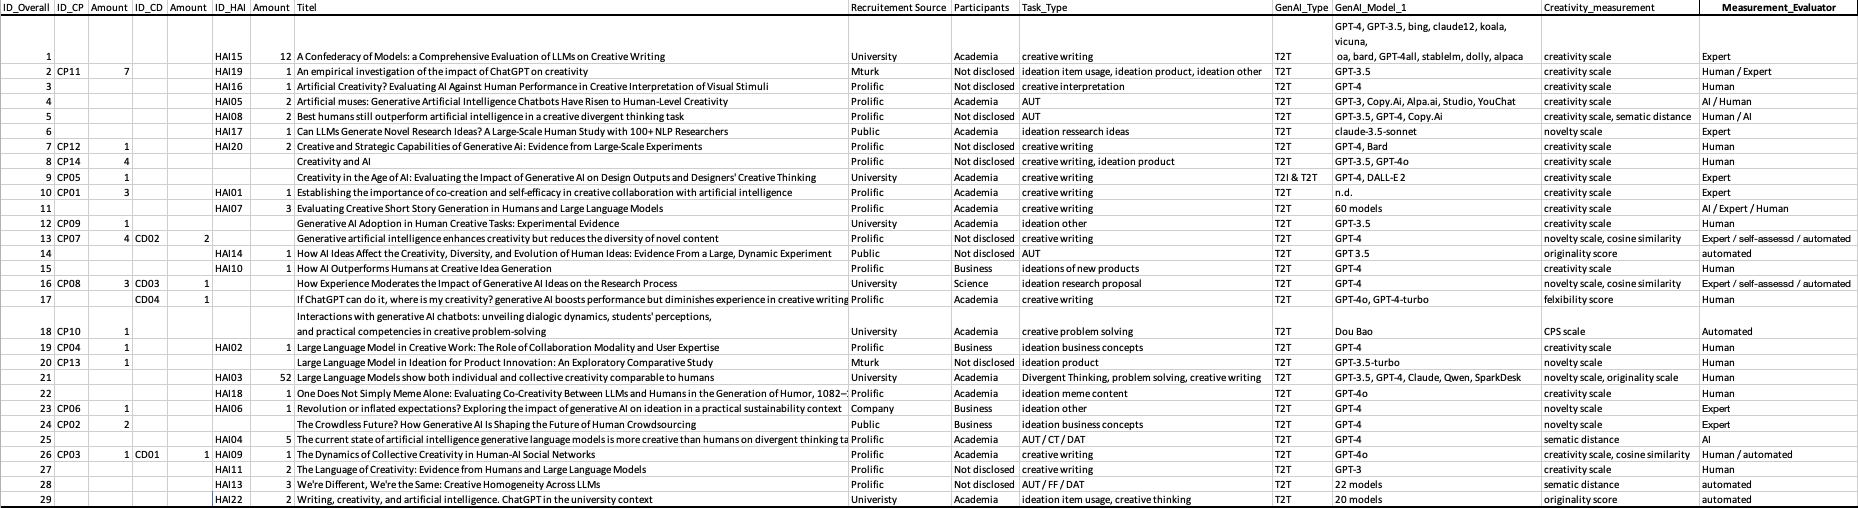
\includegraphics[width=\linewidth]{List_included_Paper.png}
  \caption{List of Literature in Review.\TODO{Umwandlung Latex Table}}
  \Description{List of Literature in Review.}
  \label{fig:TablePapers}
\end{figure}

descriptive sagen -- was machen die meisten studied für tasks (ähnlichkeiten) 

\subsection{RQ 1 :Creative Performance Comparison of Human and AI}
\label{sec:CreativePerformanceComparisonOfHumanAndAI}
\textbf{RQ 1:} How does GenAI alone compare to humans in creative performance in creativity tasks? \\
\subsubsection{Aggregated Data}
\begin{itemize}
  \item \textbf{Forest Plot:} The aggregated analysis yields a moderate positive effect ($g$ = 0.406), suggesting that GenAI creativity generally surpasses human creativity across studies. However, the wide range of confidence intervals highlights considerable variability among individual studies, implying context-dependent differences in performance.
  \item \textbf{Funnel Plot:} The funnel plot illustrates a symmetric distribution, suggesting minimal publication bias and indicating robust methodological consistency across the aggregated studies comparing human and AI creative performance.
  \item \textbf{Trim-and-Fill Funnel Plot:} The trim-and-fill procedure indicates no additional imputed studies, confirming the absence of meaningful publication bias. This further supports the reliability of the conclusion regarding GenAI's superior creative performance relative to human on the aggregate level.
  \item \textbf{Influence Diagnostics:} Influence diagnostics metrics reveal no significant influential cases or outliers. The standardized residuals, Cook’s distances, and leverage values are within normal boundaries, reinforcing the stability and generalizability of the moderate positive effect identified.
  \item \textbf{Leave-One-Out Sensitivity Analysis:} Sensitivity analysis highlights consistent stability of the pooled effect size (range $g$= 0.36 - 0.52) upon sequential exclusion of individual studies. This consistency strengthens confidence in the robustness of humans outperforming AI creatively at the aggregated study level.
\end{itemize}
\begin{figure}[H]
  \centering
  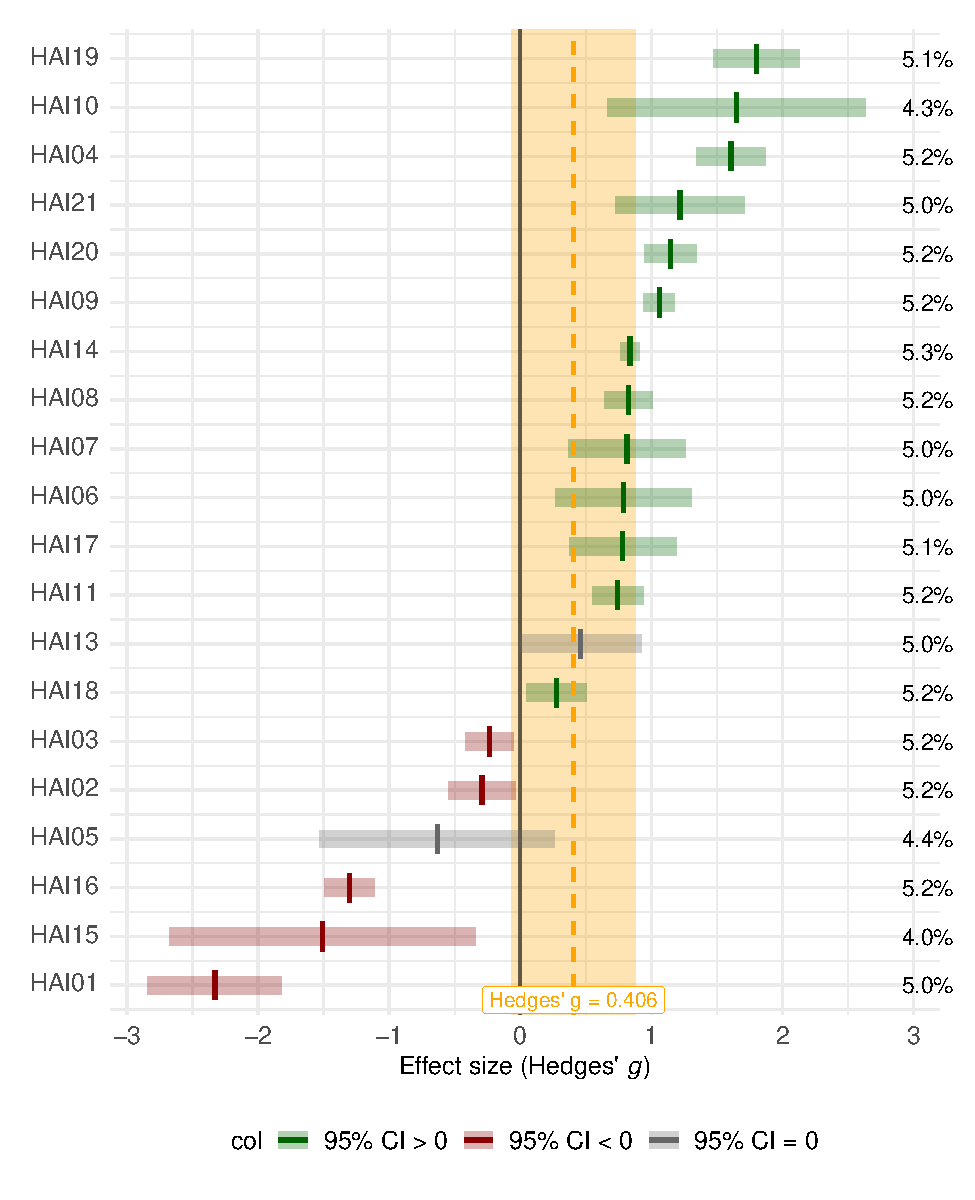
\includegraphics[width=\linewidth]{plot_versus_agg_forest}
  \caption{Forest plot summarising the Hedges’ $g$ effect sizes and 95\% confidence intervals for direct Human vs.\ AI comparison (Treatment: AI vs.\ Control: Human alone) across twenty aggregated tasks (HAI01-HAI21). Each horizontal line shows one task’s estimate (weight at right), while the central diamond shows the overall effect size of $g$ = 0.406, indicating a moderate advantage for AI outputs relative to humans. The vertical line at $g$ = 0 marks no difference; values to the right favour the AI treatment.}
  \label{fig:versus_agg_forest}
\end{figure}
\subsubsection{Raw Data}
\begin{itemize}
  \item \textbf{Forest Plot:} At the raw replication level, the effect size is negligible ($g$ = -0.050), suggesting virtually no overall difference in creative performance between humans and GenAI. The large variability and extensive overlap with zero across replications emphasize that performance is highly context-dependent and varies significantly between tasks and conditions.
  \item \textbf{Funnel Plot:}  The scatter is clearly asymmetric – small‑sample replications ($<$ $\approx$ 50 participants; SE $>$ 0.4) concentrate on the left (negative g‑values), while equivalently imprecise studies showing positive effects are virtually absent. This pattern flags a pronounced small‑study / publication bias that pulls the pooled estimate towards the negative side.
  \item \textbf{Trim-and-Fill Funnel Plot:} Inserts several right‑hand (positive) studies, and the adjusted summary line shifts upward, moving the overall g from $\approx$ -0.05 to a slightly positive value. The magnitude of the correction confirms that the raw estimate understated GenAI’s performance; publication bias or at least small‑study effects is therefore non‑negligible and must be acknowledged when interpreting RQ 1 results.
  \item \textbf{Influence Diagnostics:} Influence diagnostics demonstrate no substantially influential cases at the replication level. Metrics such as Cook’s distance and standardized residuals suggest stability and reliability, despite the high number of replications and variability observed across individual tasks and conditions.
  \item \textbf{Leave-One-Out Sensitivity Analysis:} The sensitivity analysis further supports the robustness of the negligible overall effect, revealing minimal fluctuation upon sequential exclusion of replications ($g$ $\approx$ -0.05). Thus, findings from raw data firmly suggest that, at the replication level, human and GenAI creative performances are essentially equivalent.
\end{itemize}
\begin{figure}[H]
  \centering
  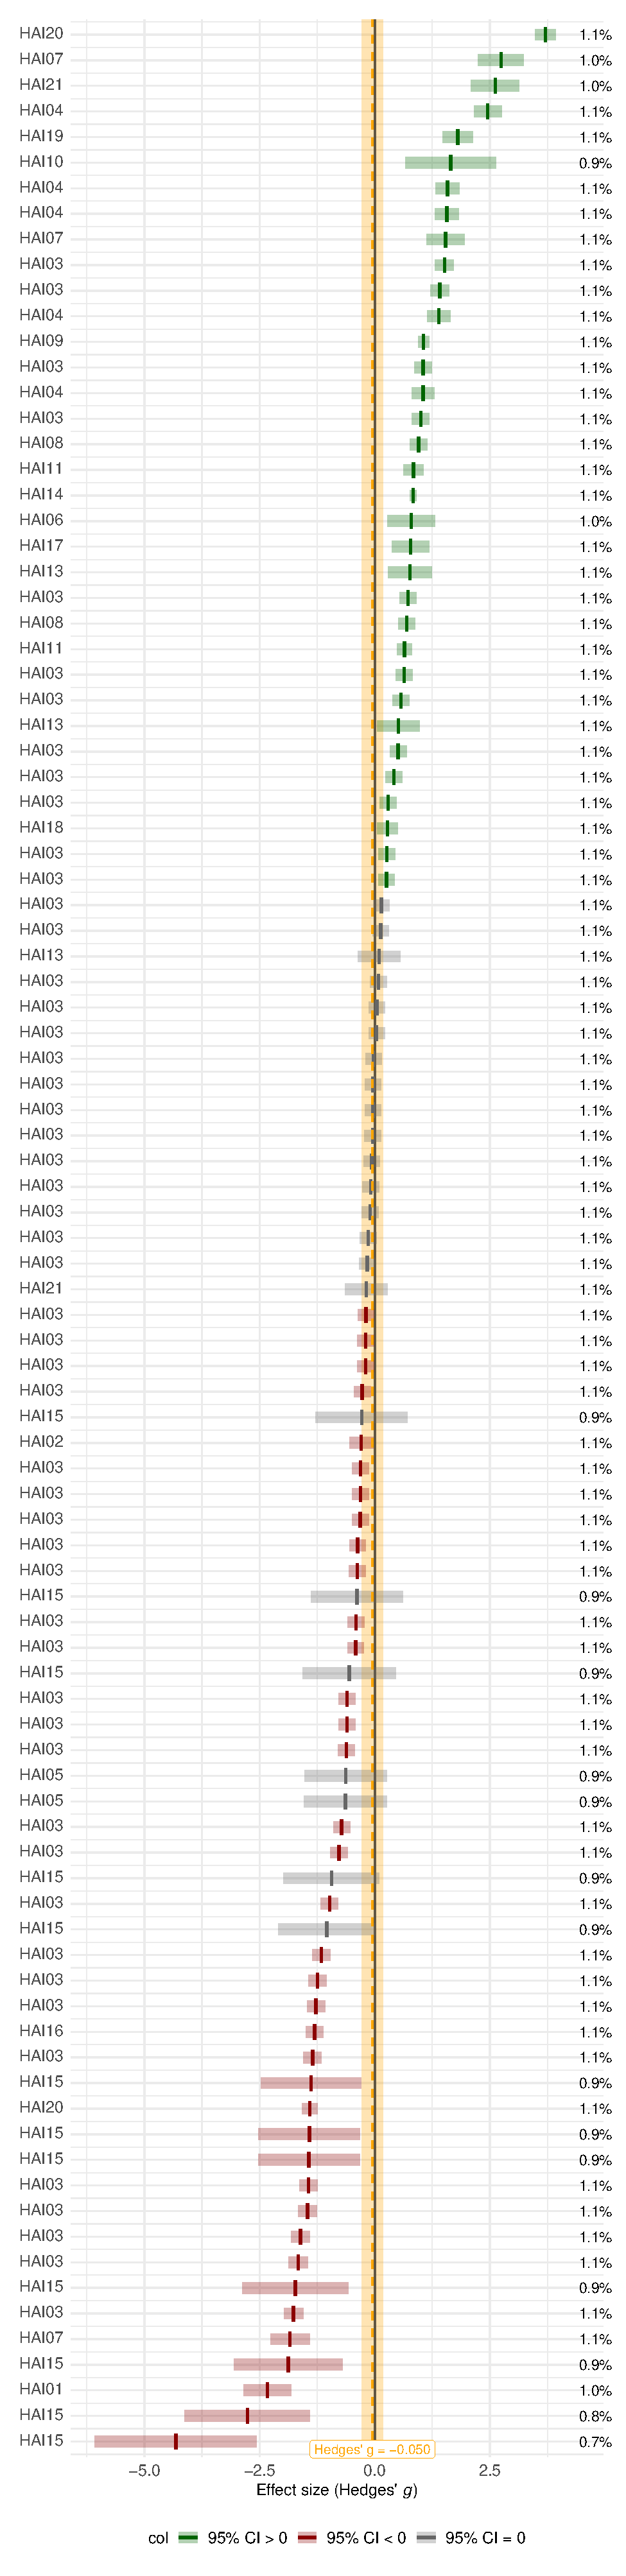
\includegraphics[width=\linewidth,
                 height=0.85\textheight,
                 keepaspectratio]{plot_versus_raw_forest}
  \caption{Forest plot summarising the Hedges’ $g$ effect sizes and 95\% confidence intervals for direct Human vs. AI comparison at the replication level (Treatment: AI vs. Control: Human alone), across multiple individual replications of HAI tasks. Each line is one replication’s estimate (weight at right), and the central diamond shows the overall effect size of $g$ = -0.050, indicating a negligible difference (slight disadvantage for AI). The vertical line at $g$ = 0 marks the null; points to the left favour the human control, to the right favour AI.}
  \label{fig:versus_raw_forest}
\end{figure}
\newpage
\subsubsection{Moderator Analysis GenAI}
\label{sec:CreativePerformanceComparisonOfHumanAndAI_Moderator_GenAI}


\begin{figure}[h]
  \centering
  % first half
  \begin{subfigure}[t]{0.49\linewidth}
    \centering
    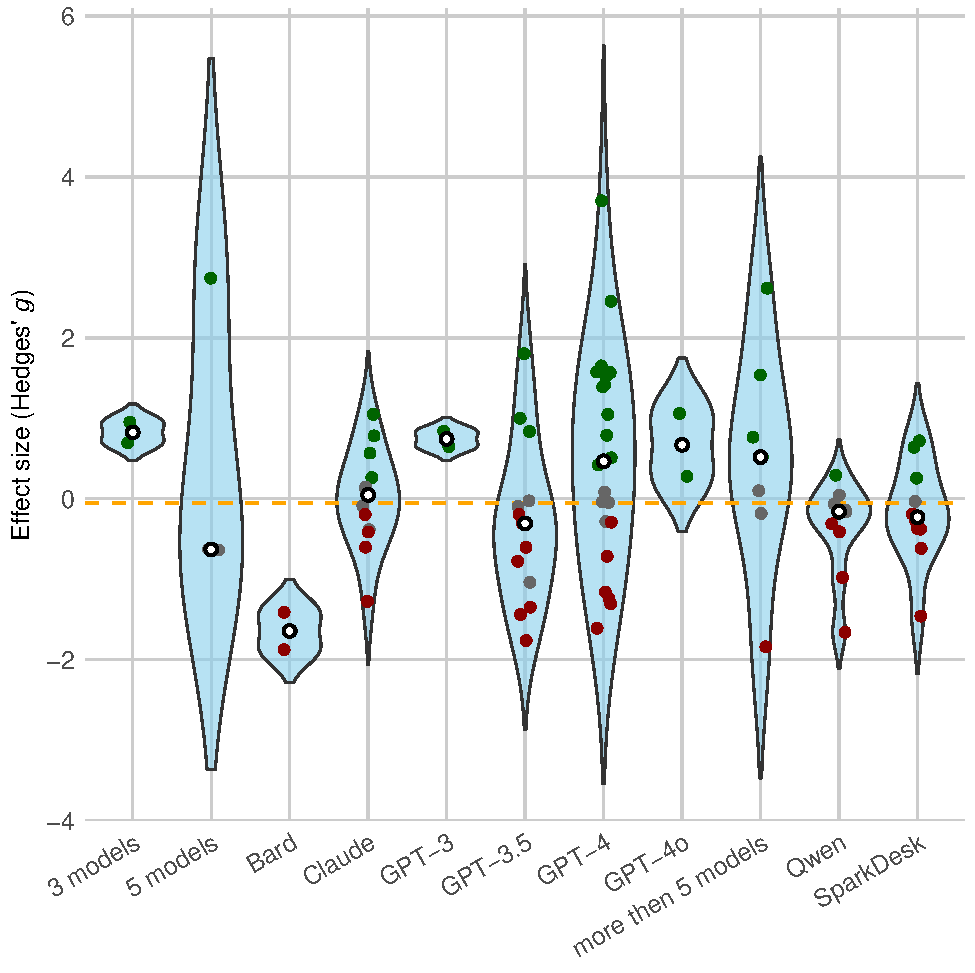
\includegraphics[width=\linewidth]{plot_versus_raw_violin_GenAI_Model}
    \caption{By model configuration.}
    \label{fig:versus_raw_violin_genai_model}
  \end{subfigure}%
  \hfill
  % second half
  \begin{subfigure}[t]{0.49\linewidth}
    \centering
    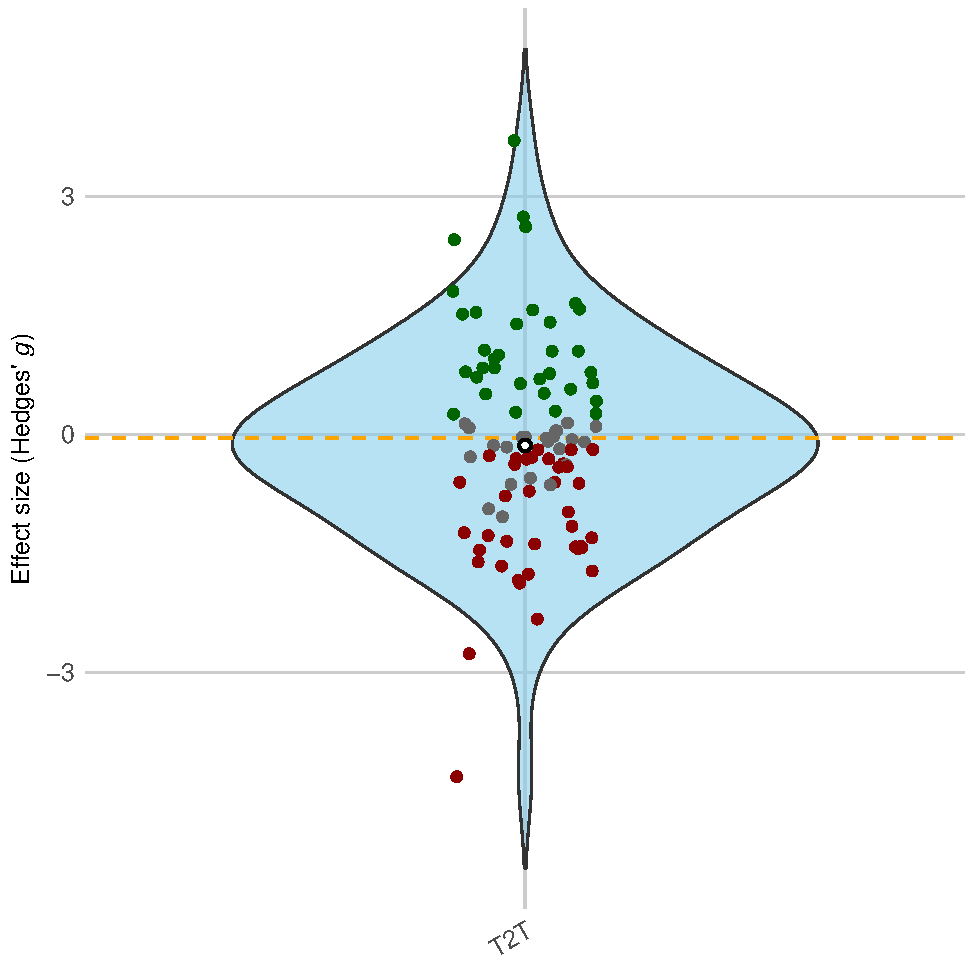
\includegraphics[width=\linewidth]{plot_versus_raw_violin_GenAI_Type}
    \caption{By interface type.}
    \label{fig:versus_raw_violin_genai_type}
  \end{subfigure}
  \caption{Violin plots showing the distribution of replication-level Hedges’ $g$ for direct Human vs.\ AI comparisons, stratified by (a) model and (b) interface type. The widths reflect density of effect sizes; $g=0$ marks no difference.}
  \label{fig:versus_raw_violins}
\end{figure}
\begin{itemize}
  \item \textbf{GenAI Type Moderator:} not executed due to <2 moderators
  \item \textbf{GenAI Type distribution:} The single available Text‑to‑Text category centres on $g$ $\approx$ 0 with symmetric spread (-3 to +3), implying that modality alone does not tilt the contest.
  \item \textbf{GenAI Model Moderator:} Only the GPT‑4 / GPT‑4o family shows a modest positive coefficient ($\approx$ +0.4-0.6), while GPT‑3/3.5 and the “3‑models / 5‑models / >5‑models” ensembles hover around zero or slightly negative; model choice therefore matters, but the advantage is confined to the latest architectures.
  \item \textbf{GenAI Model distribution:} Effect sizes are highly dispersed (-4 to +6), yet the density is thickest near 0; a long positive tail is driven by a handful of GPT‑4(o) observations, confirming the regression signal that improvements are model‑specific rather than universal.
\end{itemize}
\subsubsection{Moderator Analysis Study Setting}
\label{sec:CreativePerformanceComparisonOfHumanAndAI_Moderator_StudySetting}
\textbf{Overall implications:}
\begin{figure}[H]
  \centering
  % (a) Task Type
  \begin{subfigure}[t]{0.49\linewidth}
    \centering
    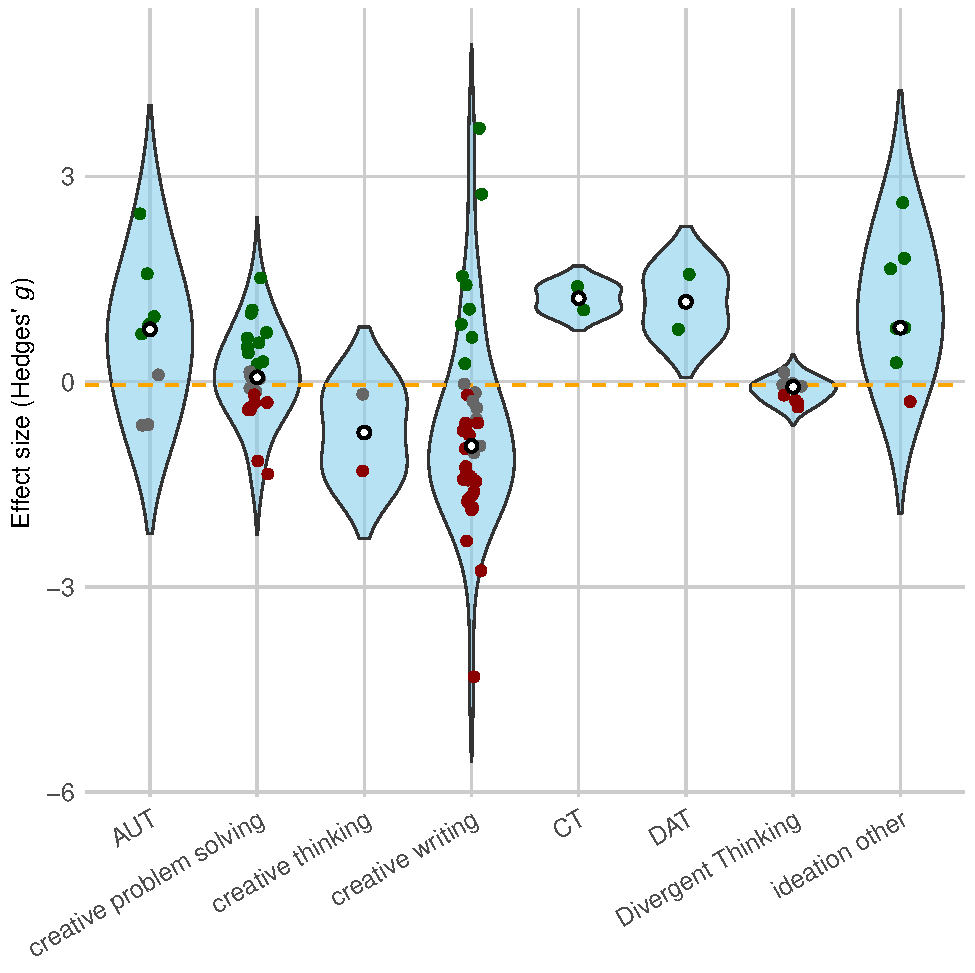
\includegraphics[width=\linewidth]{plot_versus_raw_violin_Task_Type}
    \caption{By creative task type.}
    \label{fig:versus_raw_violin_task_type}
  \end{subfigure}%
  \hfill
  % (b) Creativity Measurement
  \begin{subfigure}[t]{0.49\linewidth}
    \centering
    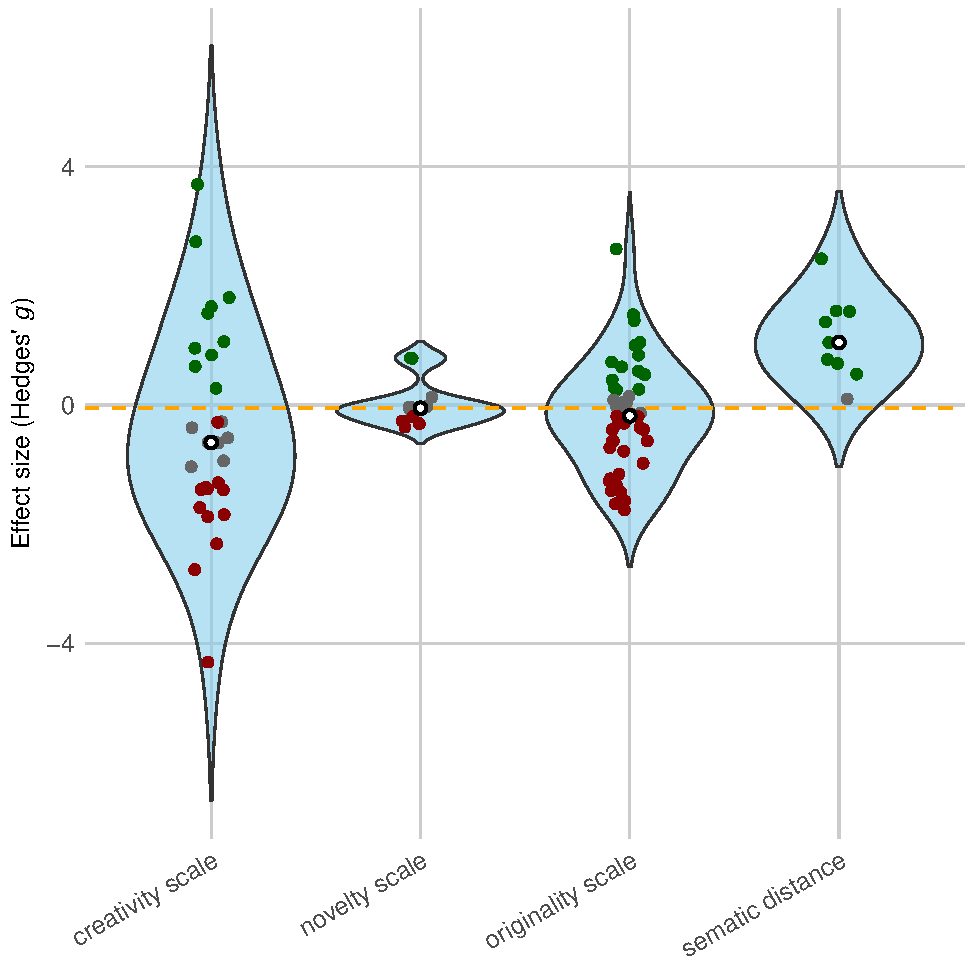
\includegraphics[width=\linewidth]{plot_versus_raw_violin_Creativity_Measurement}
    \caption{By measurement method.}
    \label{fig:versus_raw_violin_measurement}
  \end{subfigure}
  \caption{Violin plots of replication-level Hedges’ $g$ for direct Human vs.\ AI comparisons, stratified by (a) creative task type and (b) creativity measurement. Widths reflect the density of replications at each effect size; the vertical line at $g=0$ indicates no difference.}
  \label{fig:versus_raw_violins_task_measure}
\end{figure}
\begin{itemize}
  \item \textbf{Task type moderator:} Creative‑writing and divergent‑thinking tasks neutral‑to‑negative, whereas AUT, DAT and other structured ideation tasks lean positive; heterogeneity across task paradigms partly explains overall between‑study variance.
  \item \textbf{Task type distribution:} The raw violins stretch from -6 to +3, but most densities overlap around the origin, highlighting that task selection contributes variance yet no single task guarantees dominance.
  \item \textbf{Creativity measurement moderator:} Meta‑regression coefficients for all four metrics (creativity, novelty, originality scales, semantic‑distance) cluster around $g$ $\approx$ 0 with wide, overlapping CIs, so the apparent Human‑vs‑AI gap is statistically invariant to how creativity is scored.
  \item \textbf{Creativity measurement distribution:} The raw data form a balanced, almost symmetric violin spanning roughly -4 $\le$ $g$ $\le$ +4, again signalling that no single metric systematically favours either side; extreme outliers are rare and bidirectional.
\end{itemize}
\begin{figure}[H]
  \centering
  % (a) Evaluator Type
  \begin{subfigure}[t]{0.49\linewidth}
    \centering
    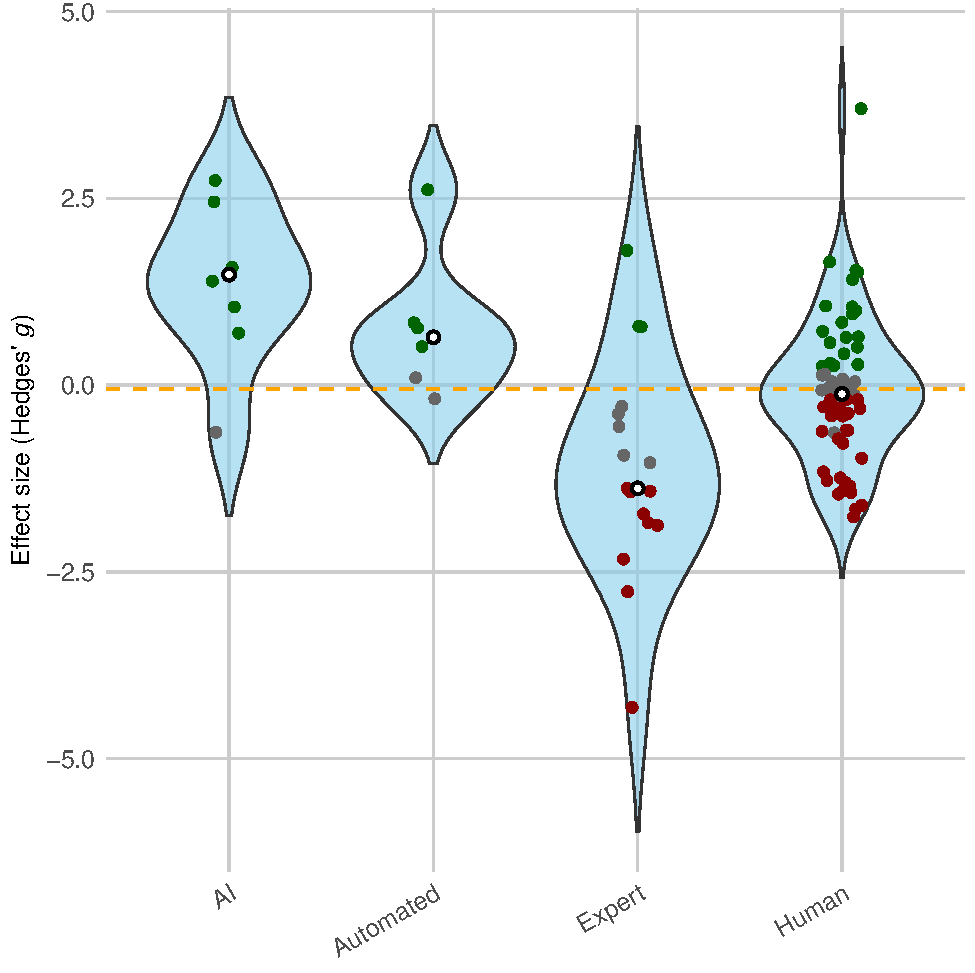
\includegraphics[width=\linewidth]{plot_versus_raw_violin_Measurement_Evaluator}
    \caption{By evaluator type (AI-automated, expert-rated, human-rated).}
    \label{fig:versus_raw_violin_evaluator}
  \end{subfigure}%
  \hfill
  % (b) Participant Source
  \begin{subfigure}[t]{0.49\linewidth}
    \centering
    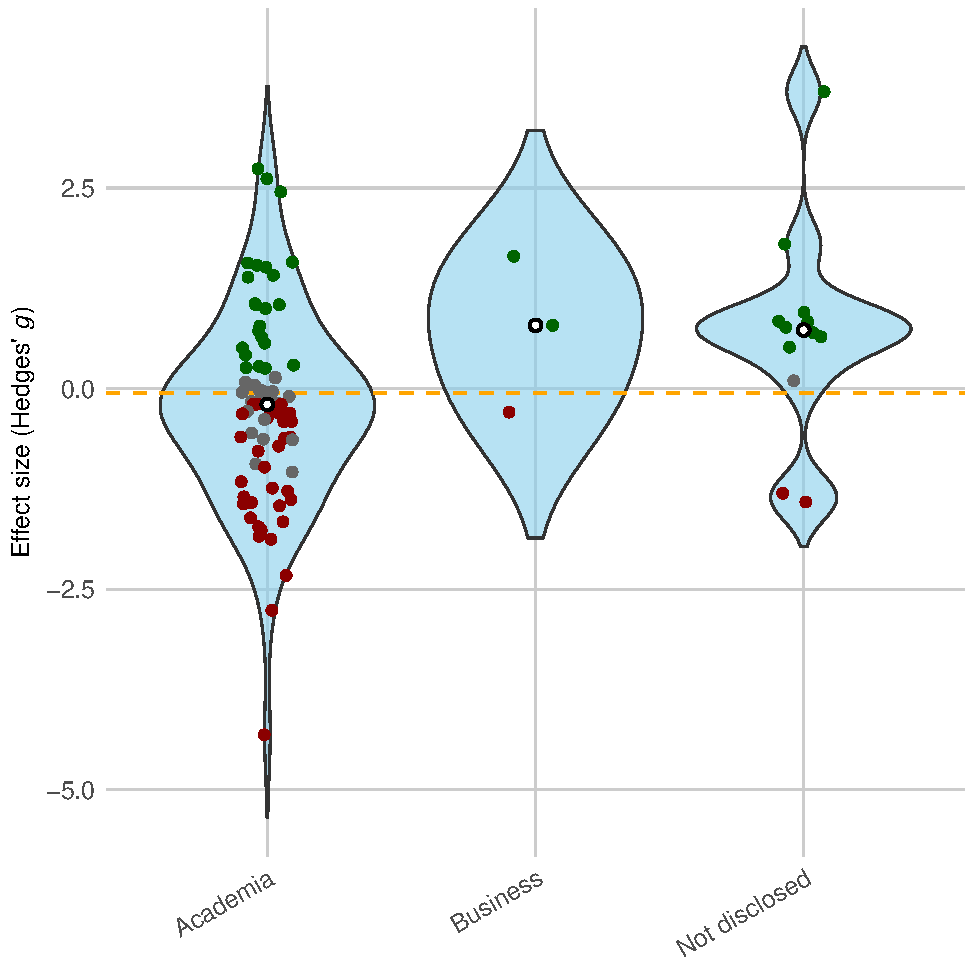
\includegraphics[width=\linewidth]{plot_versus_raw_violin_Participants}
    \caption{By participant source (academia, business, not disclosed).}
    \label{fig:versus_raw_violin_participants}
  \end{subfigure}
  \caption{Violin plots of replication-level Hedges’ $g$ for direct Human vs.\ AI comparisons, stratified by (a) evaluator type and (b) participant source. Widths reflect the density of replications at each effect size; the vertical line at $g=0$ indicates no difference.}
  \label{fig:versus_raw_violins_eval_part}
\end{figure}
\begin{itemize}
  \item \textbf{Measurement evaluator moderator:} Scores provided by AI/automated raters trend higher (positive g), whereas human experts (and general human raters) yield estimates around zero or slightly negative; who evaluates the output modestly shapes the detected gap.
  \item \textbf{Measurement evaluator distribution:} Violin widths confirm this pattern: AI/automated evaluations show a right‑skewed spread up to +5, while expert and lay‑human judgements remain tightly packed near 0, underscoring evaluator‑dependence.
  \item \textbf{Participants moderator:} Academic, business, and “not‑disclosed” samples deliver statistically indistinguishable effects; coefficients < 0.3 g and CIs overlap zero.
  \item \textbf{Participants measurement distribution:} Study‑level g spans roughly -5 to +2 in every group, with similar medians, mirroring the non‑significant moderator test.
\end{itemize}
\begin{figure}[H]
  \centering
  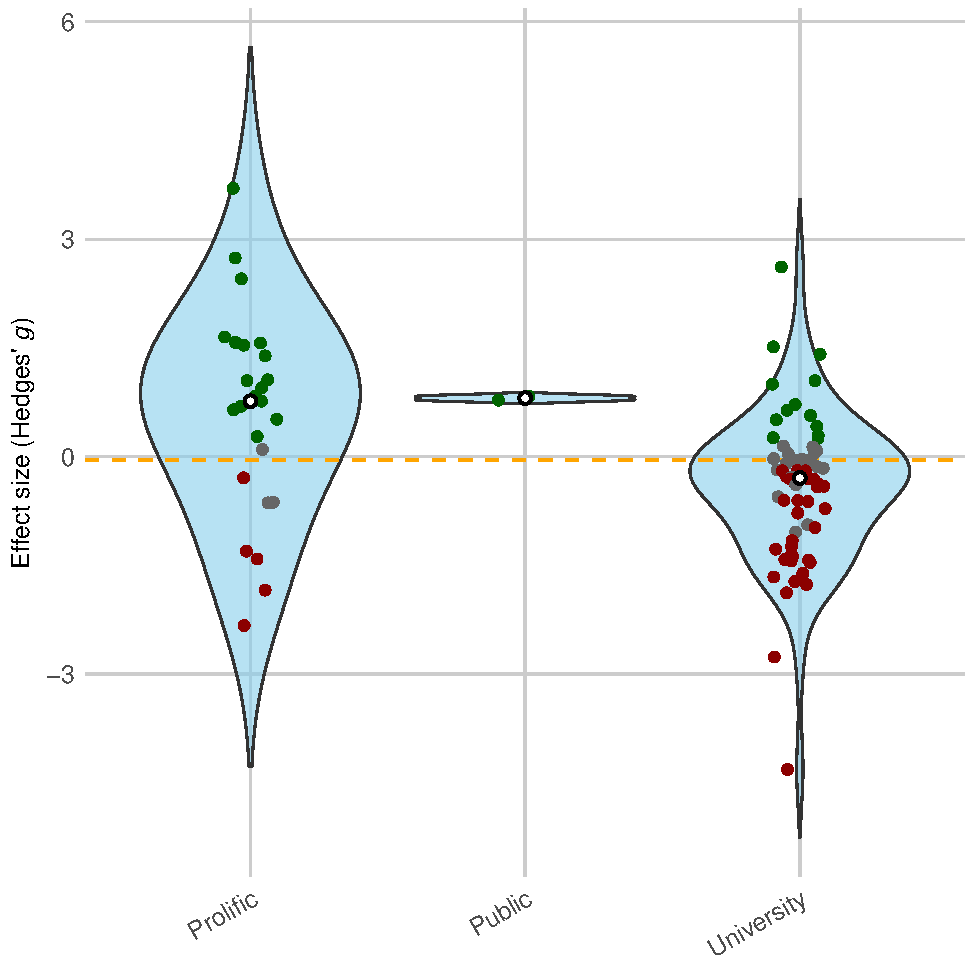
\includegraphics[width=\linewidth]{plot_versus_raw_violin_Recruitment_Source}
  \caption{Violin plot showing the distribution of replication‑level Hedges’ $g$ effect sizes for direct Human vs.\ AI comparison (Treatment: AI vs.\ Control: Human alone), stratified by recruitment source (Prolific vs.\ public vs.\ university). The violins’ densities reveal how recruitment source choice impacts the variability and magnitude of comparative effect sizes. The horizontal line at $g=0$ marks no difference.}
  \label{fig:versus_raw_violin_platform}
\end{figure}
\begin{itemize}
  \item \textbf{Recruitment source moderator:}Prolific, public‑crowd, and university pools likewise fail to predict performance differences; CIs for all coefficients include zero.
  \item \textbf{Recruitment source violin:} Central tendencies align across sources; Prolific shows a few positive outliers but overall dispersion patterns match, echoing the regression outcome.
\end{itemize}

\newpage
\subsection{RQ 2a: Creative Performance}
\label{sec:CreativePerformance}
\textbf{RQ 2a:} How does using GenAI affect human creative performance in creativity tasks? \\
\subsubsection{Aggregated Data}
\begin{itemize}
  \item \textbf{Forest Plot:} The aggregated forest plot reveals a modest positive overall effect of Human-AI collaboration on creative performance, with Hedges' $g$ = 0.164. However, several studies cross zero, indicating variability and the need for cautious interpretation of the generalizability of the effect.
  \item \textbf{Funnel Plot:} The observed funnel plot displays minor asymmetry, indicating potential publication bias or small-study effects that should be further examined to interpret the robustness of the findings accurately.
  \item \textbf{Trim-and-Fill Funnel Plot:} After applying the trim-and-fill procedure, no significant change was observed in the funnel plot. This suggests that any potential publication bias is limited and does not substantially alter the conclusion of a modest positive effect of Human-AI collaboration on creative performance.
  \item \textbf{Influence Diagnostics:} Influence diagnostics indicate no influential outliers affecting the aggregated effect size. Metrics such as Cook’s distance, residuals, and leverage remain within normal thresholds, reinforcing the stability of the reported effect.
  \item \textbf{Leave-One-Out Sensitivity Analysis:} Sensitivity analysis demonstrates minimal variability in the aggregated effect size upon the sequential exclusion of individual studies, confirming robustness and reliability of the modest positive effect identified (range $g$ = 0.14 - 0.20).
\end{itemize}
\begin{figure}[H]
  \centering
  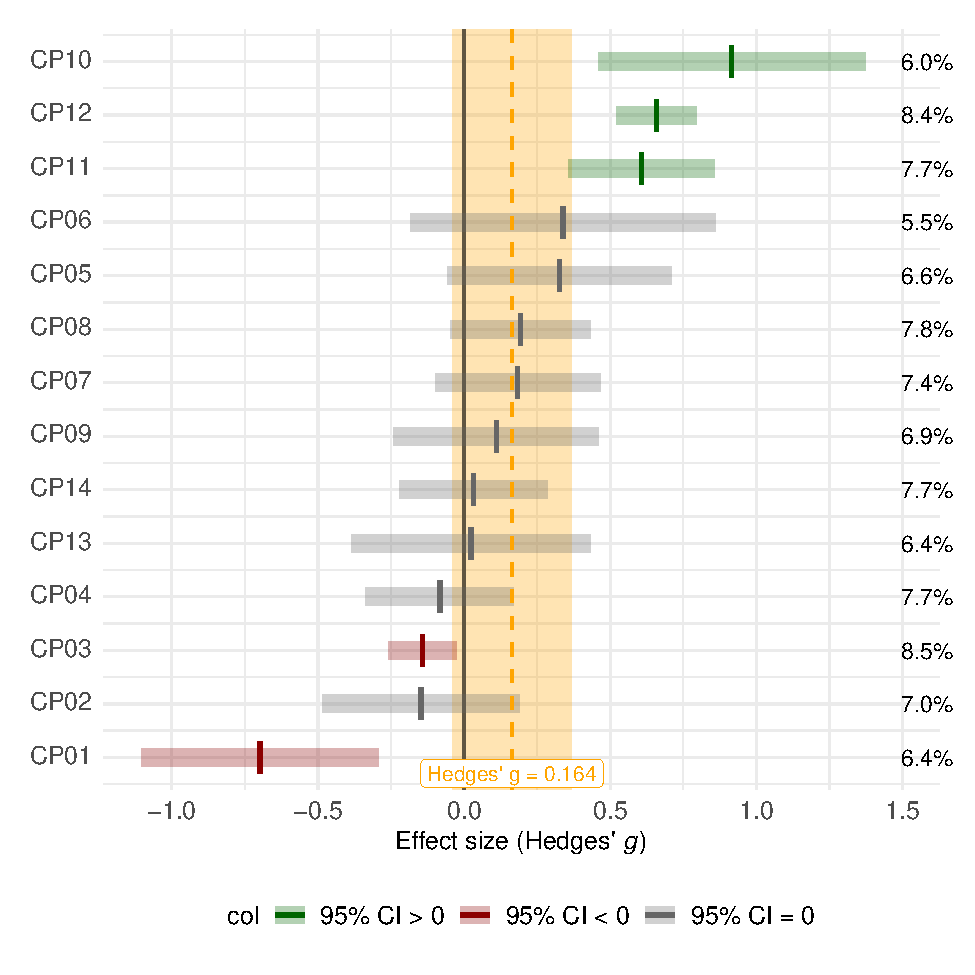
\includegraphics[width=\linewidth]{plot_performance_agg_forest}
  \caption{Forest plot summarising the Hedges’ $g$ effect sizes and 95\% confidence intervals for creative performance (Treatment: Human+AI vs. Control: Human alone) across fourteen aggregated tasks (CP01-CP14). Each horizontal line shows one task’s estimate (weight at right), while the central diamond shows the overall effect size of $g$ = 0.185, indicating a small but consistent performance boost when humans are assisted by AI. The vertical line at $g$ = 0 marks no difference; estimates to the right favour the AI‑assisted treatment.}
  \label{fig:performance_agg_forest}
\end{figure}
\subsubsection{Raw Data}
\begin{itemize}
  \item \textbf{Forest Plot:} The raw replication-level forest plot confirms a consistent, although small, positive overall effect of Human-AI collaboration on creative performance, with Hedges' $g$ = 0.180. While positive, variability among individual replications is evident, suggesting context-dependent effectiveness.
  \item \textbf{Funnel Plot:} The funnel plot for the raw data illustrates moderate asymmetry, potentially indicating publication bias or methodological heterogeneity at the replication level, which necessitates further detailed exploration.
  \item \textbf{Trim-and-Fill Funnel Plot:} Application of the trim-and-fill method to the raw data does not markedly change the funnel plot, suggesting the observed asymmetry has limited impact on the overall conclusions of modest positive effects.
  \item \textbf{Influence Diagnostics:} Diagnostic metrics such as Cook's distance and standardized residuals for the raw data remain largely acceptable, confirming no single replication disproportionately influences the overall positive effect estimation. However, some minor variability indicates replication-specific nuances.
  \item \textbf{Leave-One-Out Sensitivity Analysis:} The leave-one-out analysis confirms the robustness of the pooled effect size (consistently around $g$ $\approx$ 0.18), further validating the conclusion that the positive impact of Human-AI collaboration on creative performance is resilient to the exclusion of individual studies.
\end{itemize}
\begin{figure}[H]
  \centering
  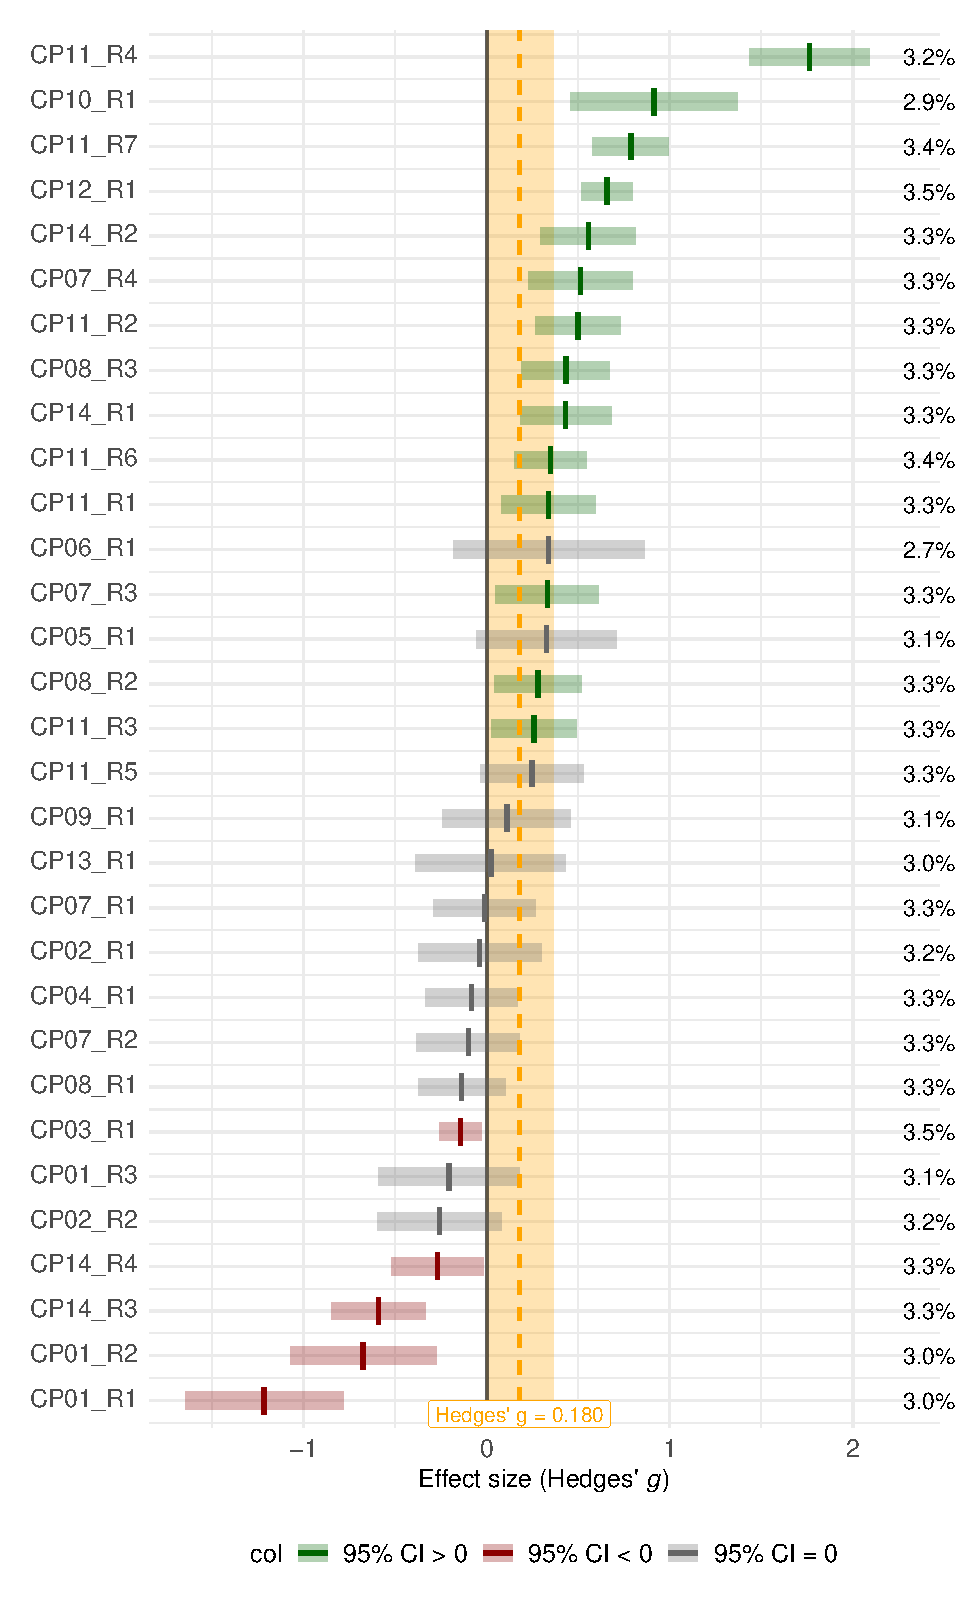
\includegraphics[width=\linewidth,
                 height=0.9\textheight,
                 keepaspectratio]{plot_performance_raw_forest}
  \caption{Forest plot summarising the Hedges’ $g$ effect sizes and 95\% confidence intervals for creative performance at the replication level (Treatment: Human+AI vs Control: Human alone), across multiple replication trials for the fourteen tasks (e.g. CP01\_R1-CP14\_R4). Each line is one trial’s estimate (weight at right), and the central diamond shows the overall effect size of $g$ = 0.219, indicating a modest performance gain from AI assistance. The vertical line at $g$ = 0 marks no effect; points to the right favour the AI‑assisted treatment.}
  \label{fig:performance_raw_forest}
\end{figure}

\subsubsection{Moderator Analysis GenAI}
\label{sec:CreativePerformance_Moderator_GenAI}
\begin{figure}[H]
  \centering
  % (a) Generative AI Model
  \begin{subfigure}[t]{0.49\linewidth}
    \centering
    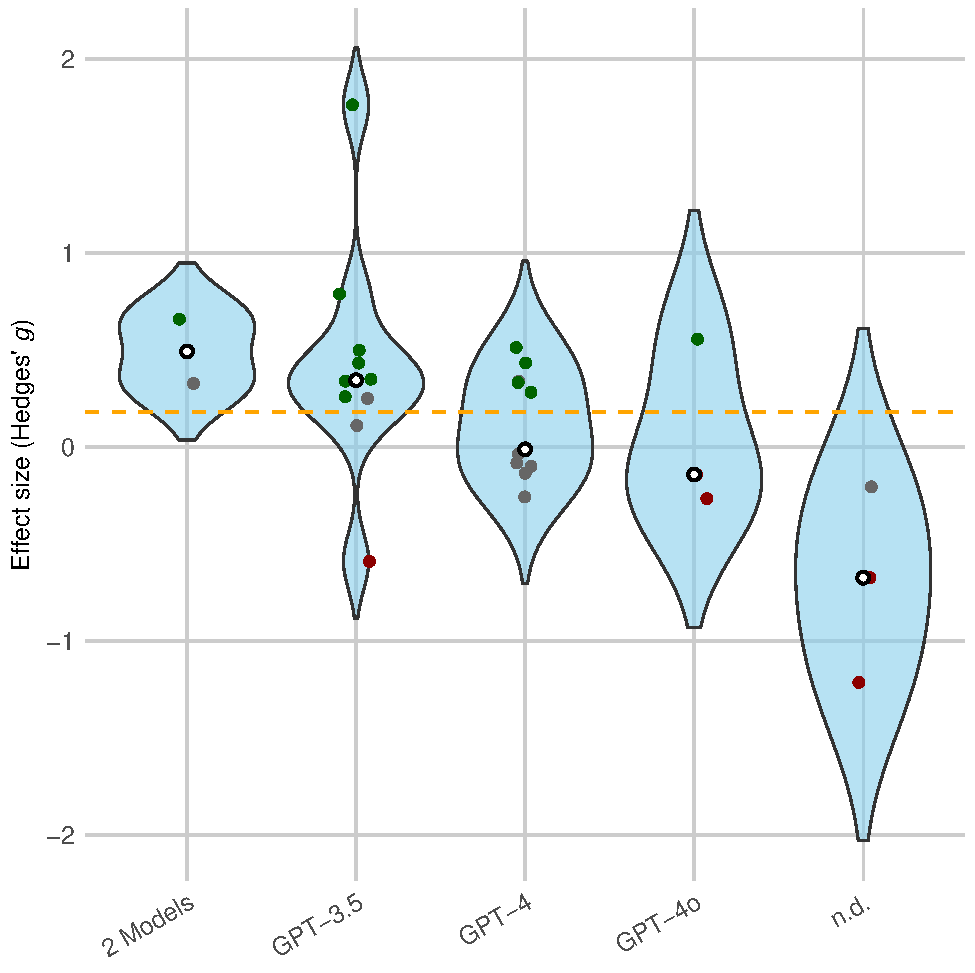
\includegraphics[width=\linewidth]{plot_performance_raw_violin_GenAI_Model}
    \caption{By generative AI model (e.g.\ GPT-3.5, GPT-4, GPT-4o).}
    \label{fig:performance_raw_violin_genai_model}
  \end{subfigure}%
  \hfill
  % (b) Generative AI Type
  \begin{subfigure}[t]{0.49\linewidth}
    \centering
    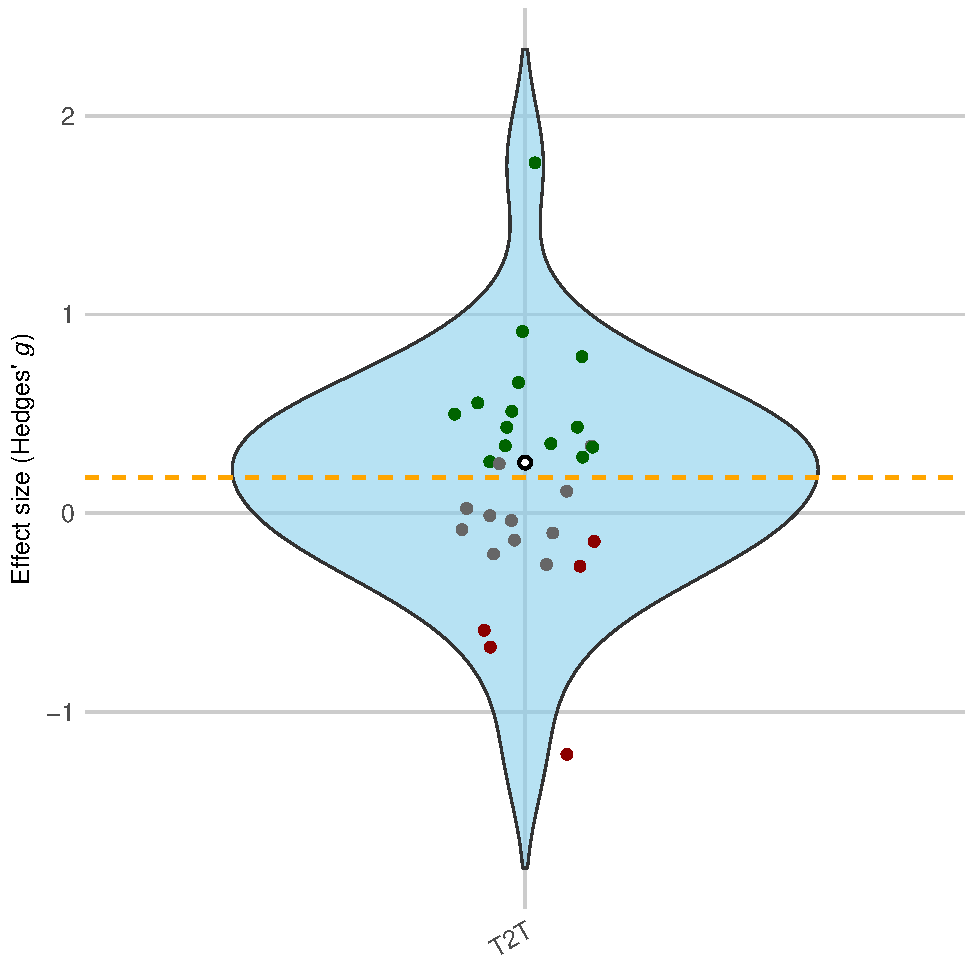
\includegraphics[width=\linewidth]{plot_performance_raw_violin_GenAI_Type}
    \caption{By generative AI type (e.g.\ text-to-text).}
    \label{fig:performance_raw_violin_genai_type}
  \end{subfigure}
  \caption{Violin plots of replication-level Hedges’ $g$ for creative performance (Treatment: Human+AI vs.\ Control: Human alone), stratified by (a) AI model and (b) AI interface type. Widths reflect the density of replications at each effect size.}
  \label{fig:performance_raw_violins_genai}
\end{figure}
\begin{itemize}
  \item \textbf{GenAI Type Moderator:} not executed due to <2 moderators
  \item \textbf{GenAI Type distribution:} T2T studies span the full effect‑size spectrum ($\approx$ -1 $g$ to +2 g) with a median near zero, mirroring the inconclusive moderator result.
  \item \textbf{GenAI Model Moderator:} Point‑estimates vary from slightly negative for the “2‑model” setups ($\approx$ -0.30 $g$) to modestly positive for GPT‑4 ($\approx$ +0.25 $g$), yet every confidence band overlaps zero, so no single foundation model outperforms the others at the aggregate level.
  \item \textbf{GenAI Model distribution:} Individual‐study effects are highly dispersed within each model family (range $\approx$ -1.5 $g$ to +1.5 $g$), underscoring that model choice alone does not explain variance in creative‑performance outcomes.
\end{itemize}
\subsubsection{Moderator Analysis Study Setting}
\label{sec:CreativePerformance_Moderator_Study_Setting}
\begin{figure}[H]
  \centering
  % (a) Creative Task Type
  \begin{subfigure}[t]{0.49\linewidth}
    \centering
    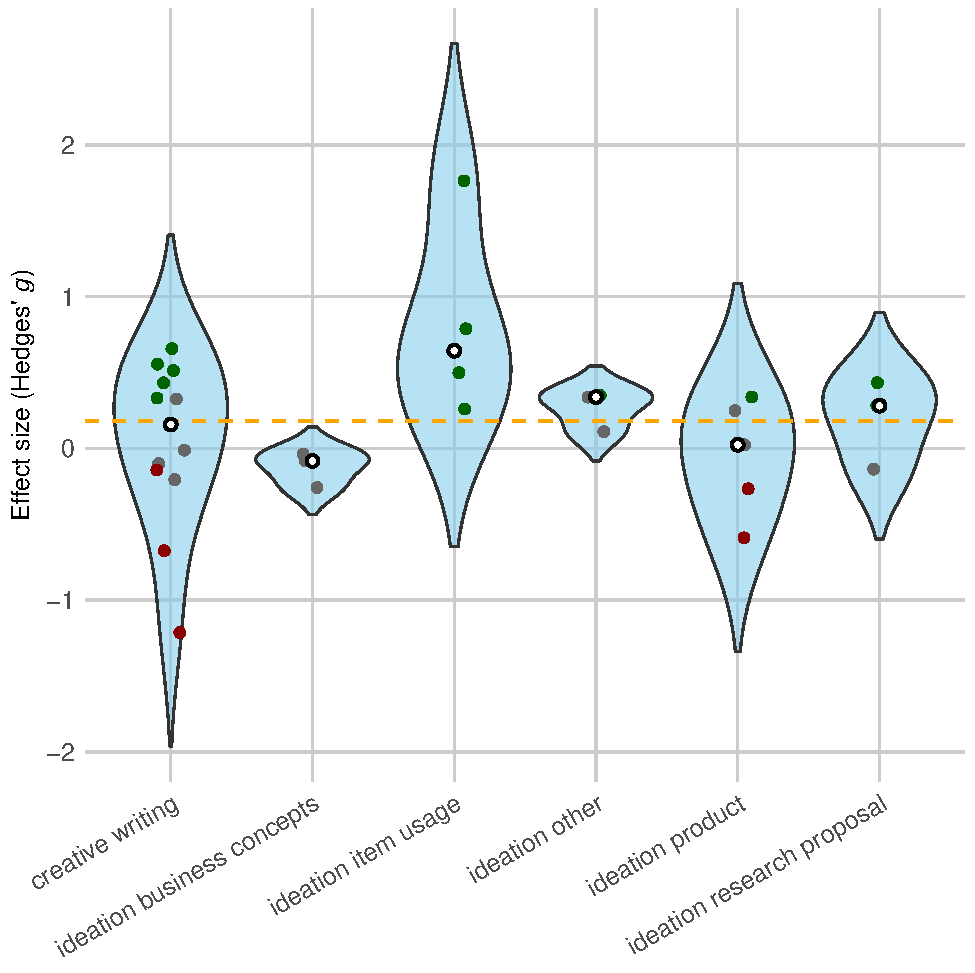
\includegraphics[width=\linewidth]{plot_performance_raw_violin_Task_Type}
    \caption{By creative task type (writing, business ideation, item usage, product concepts, research proposals).}
    \label{fig:performance_raw_violin_task_type}
  \end{subfigure}%
  \hfill
  % (b) Creativity Measurement
  \begin{subfigure}[t]{0.49\linewidth}
    \centering
    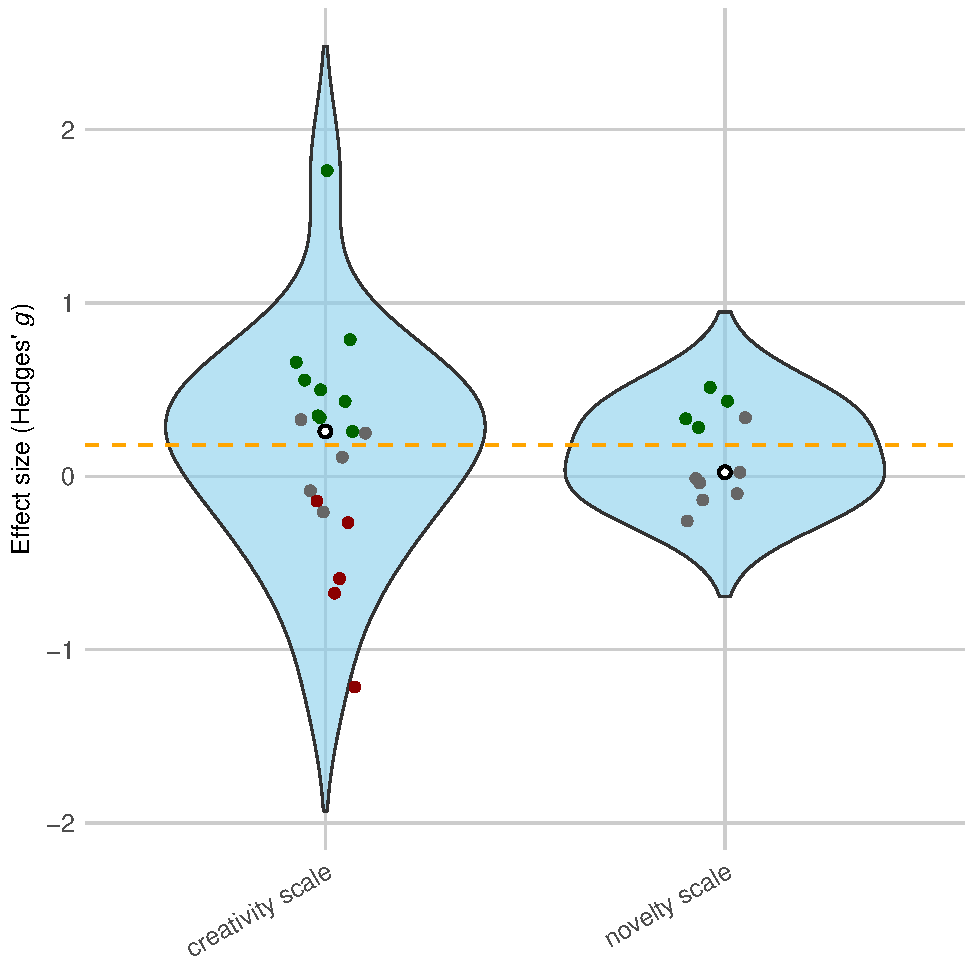
\includegraphics[width=\linewidth]{plot_performance_raw_violin_Creativity_Measurement}
    \caption{By measurement method (creativity vs.\ novelty scale).}
    \label{fig:performance_raw_violin_measurement}
  \end{subfigure}
  \caption{Violin plots of replication-level Hedges’ $g$ for creative performance (Human+AI vs.\ Human alone), stratified by (a) task domain and (b) measurement metric. Widths reflect the density of effect sizes across replications.}
  \label{fig:performance_raw_violins_task_measure}
\end{figure}
\begin{itemize}
  \item \textbf{Task type moderator:} None of the six creative‑task categories (e.g., creative writing, product ideation) produced a significant deviation from the grand mean; the largest point‑estimate (business‑concept ideation, $\approx$ +0.40 $g$) still crossed zero. 
  \item \textbf{Task type distribution:} Effect‑size distributions for all task categories overlap extensively, with medians hovering around the null, signalling that task selection alone cannot account for performance heterogeneity.
  \item \textbf{Creativity measurement moderator:} Neither the creativity nor the novelty rating scales meaningfully shifted the pooled performance effect (point‑estimates $\approx$ 0.10-0.15, 95 \% CIs straddle 0), indicating measurement choice did not moderate Gen‑AI performance gains.
  \item \textbf{Creativity measurement distribution:} Raw study effects cluster tightly around zero for both rating scales, with a few positive and negative outliers, visually reinforcing the absence of systematic measurement bias.
\end{itemize}
\begin{figure}[H]
  \centering
  % (a) Evaluator Type
  \begin{subfigure}[t]{0.49\linewidth}
    \centering
    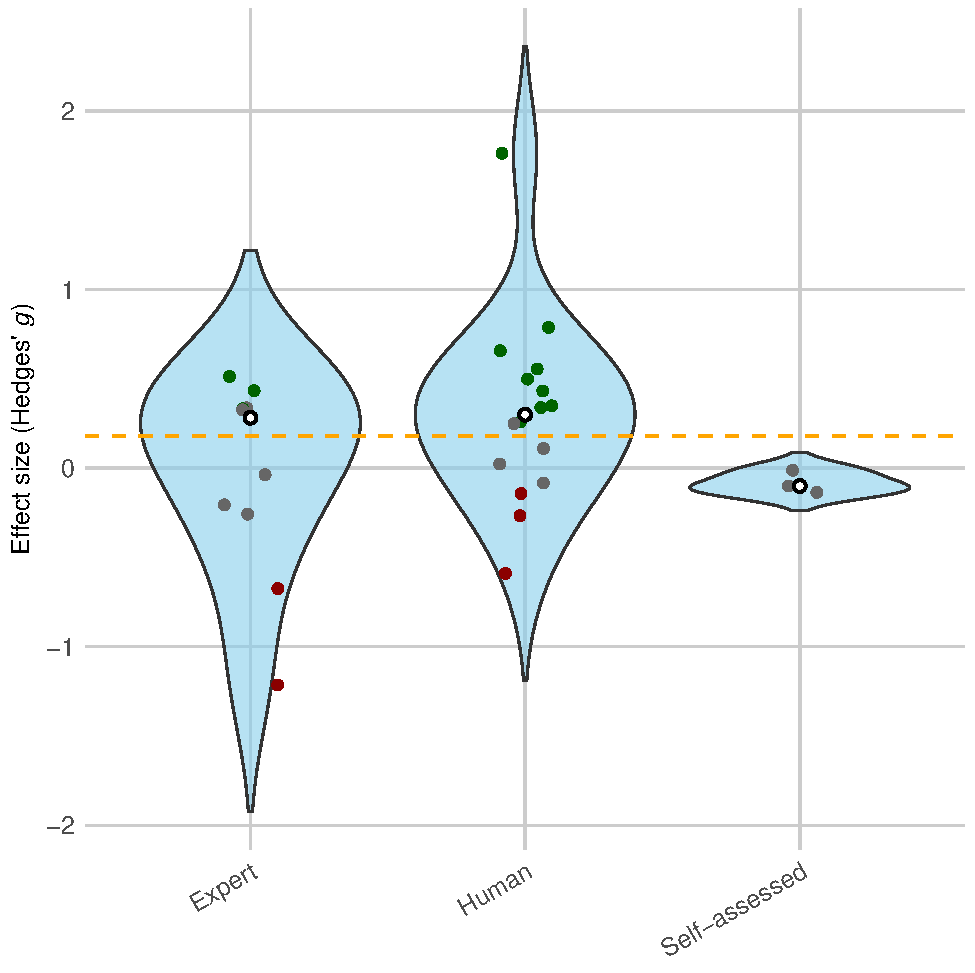
\includegraphics[width=\linewidth]{plot_performance_raw_violin_Measurement_Evaluator}
    \caption{By evaluator type (expert-rated, human-rated, self-assessed).}
    \label{fig:performance_raw_violin_evaluator}
  \end{subfigure}%
  \hfill
  % (b) Participant Source
  \begin{subfigure}[t]{0.49\linewidth}
    \centering
    \includegraphics[width=\linewidth]{plot_performance_raw_violin_participants}
    \caption{By participant source (academia, business, science, not disclosed).}
    \label{fig:performance_raw_violin_participants}
  \end{subfigure}
  \caption{Violin plots of replication-level Hedges’ $g$ for creative performance (Human+AI vs.\ Human alone), stratified by (a) evaluator type and (b) participant source. Die Breiten spiegeln die Dichte der Effektgrößen wider.}
  \label{fig:performance_raw_violins_eval_part}
\end{figure}
\begin{itemize}
  \item \textbf{Measurement evaluator moderator:} Whether outputs were scored by experts, lay humans, or self‑assessment showed negligible, non‑significant differences (coefficients within ±0.15 $g$), indicating evaluation source did not bias reported performance.
  \item \textbf{Measurement evaluator distribution:} All three evaluator groups display similarly wide and overlapping effect‑size spreads, supporting the lack of systematic evaluation bias.
  \item \textbf{Participants moderator:} Neither academia, business professionals, scientists, nor studies with undisclosed samples show a statistically reliable deviation from the grand‑mean effect (all 95 \% CIs overlap zero; |$g$| < 0.3), indicating that the performance boost of GenAI is not contingent on participants’ occupational background.
  \item \textbf{Participants measurement distribution:} The violin plot confirms the meta‑regression: all four groups exhibit wide, largely overlapping distributions centred close to zero. Extreme positive and negative outliers are scarce and balanced, underscoring the absence of systematic between‑group differences.
\end{itemize}
\begin{figure}[H]
  \centering
  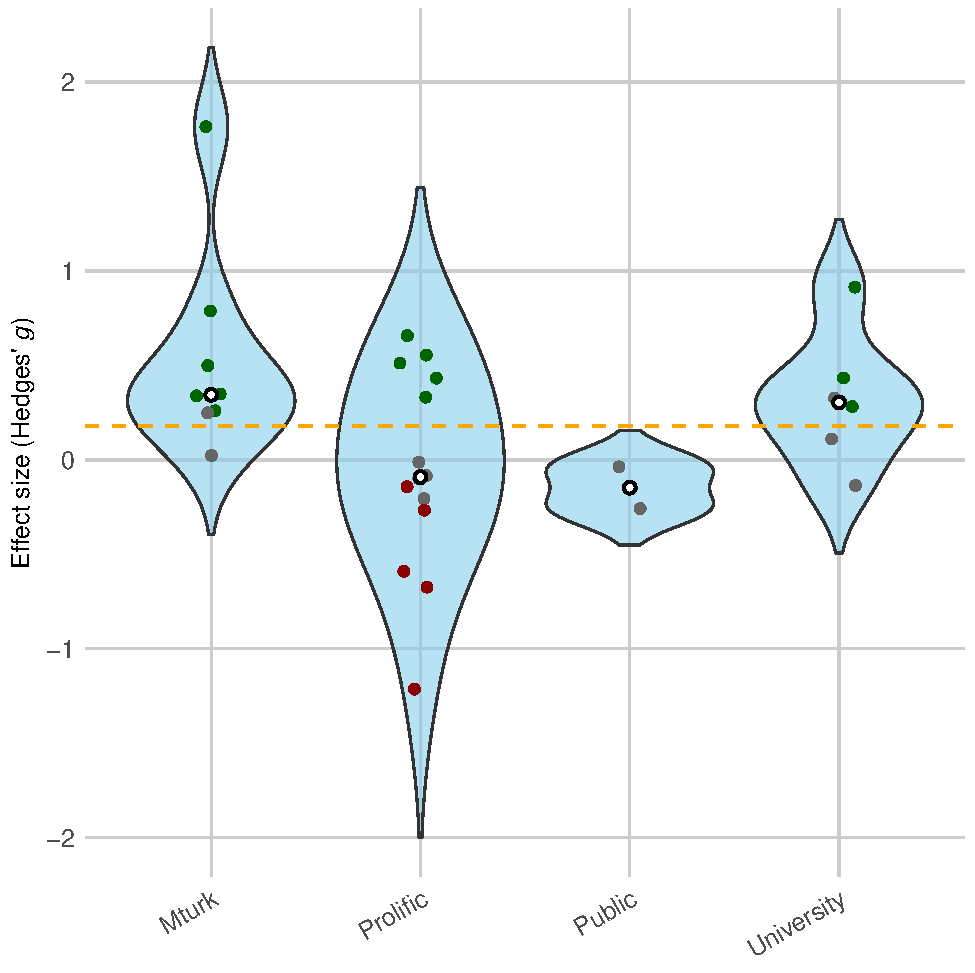
\includegraphics[width=\linewidth]{plot_performance_raw_violin_Recruitment_Source}
  \caption{Violin plot showing the distribution of replication‑level Hedges’ $g$ effect sizes for creative performance (Treatment: Human+AI vs.\ Control: Human alone), stratified by recruitment recruitment source (MTurk, Prolific, public, university). The violins’ densities reveal how recruitment source choice impacts the variability and magnitude of performance gains.}
  \label{fig:performance_raw_violin_Recruitment_Source}
\end{figure}
\begin{itemize}
  \item \textbf{Recruitment source moderator:} Effect estimates for samples drawn from MTurk, Prolific, public calls, and university pools likewise cluster tightly around the overall average (|$g$| $\lesssim$ 0.2; CIs span zero), suggesting that data‑collection platform does not moderate GenAI‑driven creative‑performance gains.
  \item \textbf{Recruitment source violin:} The corresponding violin plot mirrors the regression outcome: each recruitment channel displays a broad but symmetrical spread of study‑level effects, with medians close to the null and no platform exhibiting a consistently beneficial or detrimental pattern.
\end{itemize}
\newpage
\subsection{RQ 2b :Creative Diversity}
\label{sec:CreativeDiversity}

\textbf{RQ 2b:} How does using GenAI affect idea diversity in creativity tasks? \\

\textbf{Strong limitation due to small amount of studies available}
\subsubsection{Aggregated Data}
\begin{itemize}
  \item \textbf{Forest Plot:} The aggregated effect size indicates a robust positive effect (Hedges' $g$ = 0.760), suggesting a significant improvement in creative diversity when using Human-AI co-creativity compared to human-only creativity. All studies included exhibit positive effect sizes with confidence intervals above zero, reinforcing this finding.
  \item \textbf{Influence Diagnostics:} Influence diagnostics indicate no substantial outliers or overly influential data points in the aggregated dataset. Cook's distances and standardized residuals are well within acceptable ranges, supporting the stability and reliability of the overall estimated effect.
  \item \textbf{Leave-One-Out Sensitivity Analysis:} Sensitivity analysis confirms the stability of the pooled effect size; omitting any single study does not significantly alter the overall result. Thus, the finding of a positive effect on creative diversity from Human-AI collaboration remains consistent and robust across all studies.
\end{itemize}
\begin{figure}[H]
  \centering
  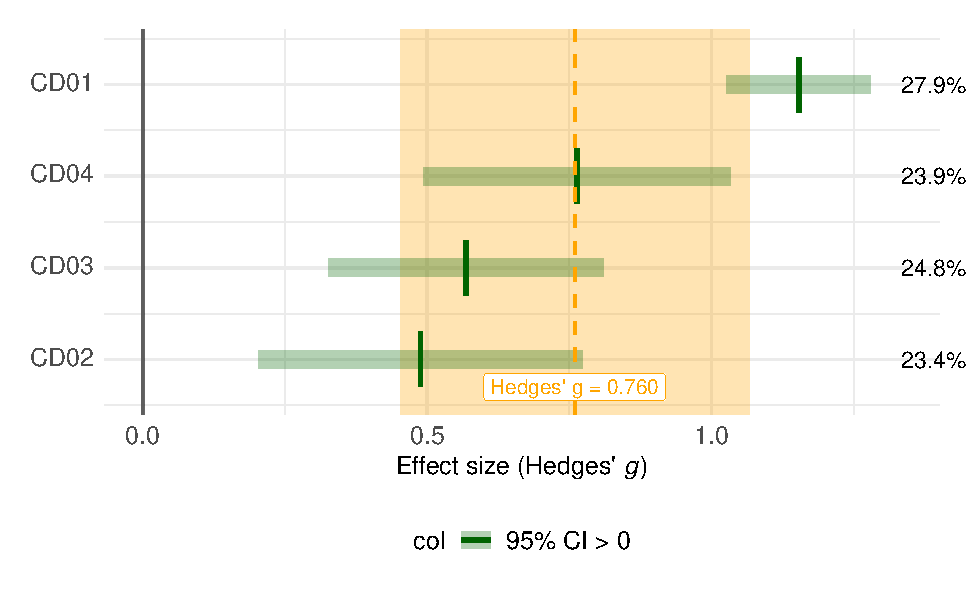
\includegraphics[width=\linewidth]{plot_diversity_agg_forest}
  \caption{Forest plot summarising the Hedges’ $g$ effect sizes and 95\% confidence intervals for creative diversity (Treatment: Human+AI vs. Control: Human alone) across four aggregated datasets (CD01-CD04). Each horizontal line shows one dataset’s point estimate (with its sample‑specific weight noted at the right), and the central diamond shows the overall summary effect size of $g$ = 2.557, indicating a large boost in diversity when humans collaborate with AI compared to working alone. The vertical line at $g$ = 0 marks no difference; values to the right favour the AI‑assisted treatment, while values to the left would favour the human‑only control.}
  \label{fig:diversity_agg_forest}
\end{figure}
\subsubsection{Raw Data}
\begin{itemize}
  \item \textbf{Forest Plot:} The raw data analysis yields a similarly positive and substantial effect (Hedges' $g$ = 0.709), indicating that even at the individual replication level, the integration of AI consistently enhances creative diversity across multiple contexts and replications.
  \item \textbf{Influence Diagnostics:} Influence diagnostics for the raw dataset reveal no critical influential points or outliers. The calculated metrics, including Cook’s distance and studentized residuals, are within acceptable limits, ensuring that no single replication disproportionately impacts the overall effect size estimation.
  \item \textbf{Leave-One-Out Sensitivity Analysis:} Leave-one-out sensitivity analyses demonstrate minor variability, with pooled estimates consistently above $g$ = 0.65. Thus, the effect of Human-AI collaboration on creative diversity is resilient and insensitive to individual study removal, further validating the generalizability of these results.
\end{itemize}
\begin{figure}[H]
  \centering
  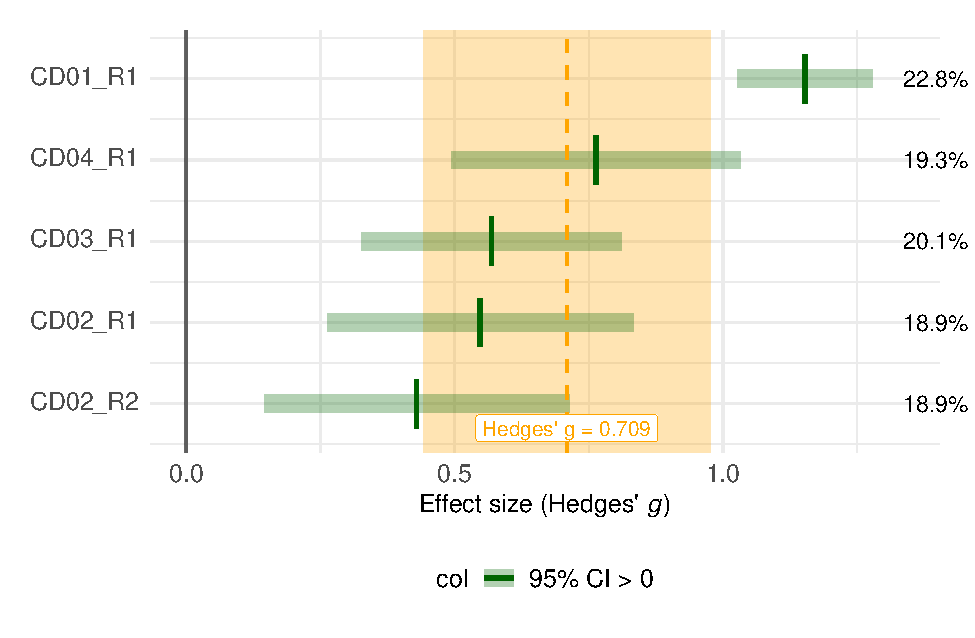
\includegraphics[width=\linewidth]{plot_diversity_raw_forest}
  \caption{Forest plot summarising the Hedges’ $g$ effect sizes and 95\% confidence intervals for creative diversity at the replication level (Treatment: Human+AI vs. Control: Human alone), across five individual replications (CD01\_R1, CD02\_R1, CD02\_R2, CD03\_R1, CD04\_R1). Each line is one replication’s estimate (weight at right), and the central diamond is the overall effect size of $g$ = 2.139, indicating a substantial diversity gain from AI assistance. The vertical line at $g$ = 0 marks the null—rightwards points favour the AI‑assisted treatment.}
  \label{fig:diversity_raw_forest}
\end{figure}

\subsubsection{Moderator Analysis GenAI}
\label{sec:CreativeDiversity_Moderator_GenAI}
\begin{figure}[H]
  \centering
  % (a) Generative AI Model
  \begin{subfigure}[t]{0.49\linewidth}
    \centering
    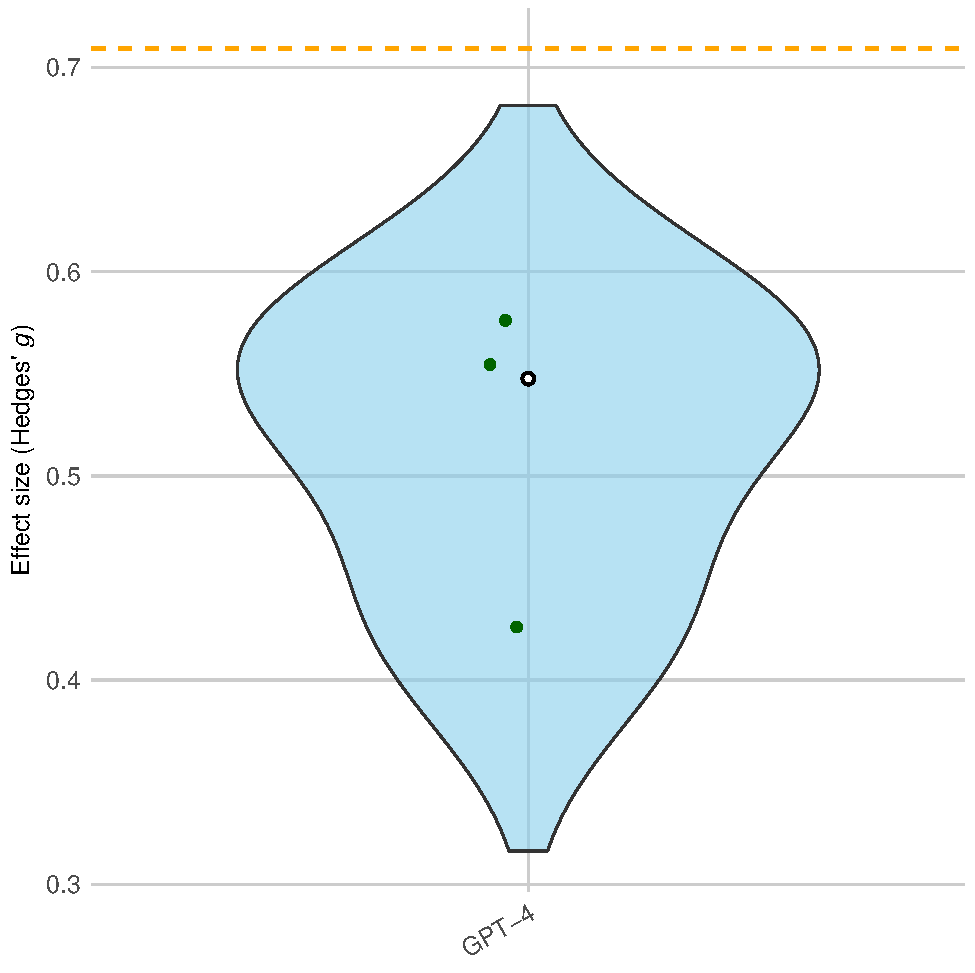
\includegraphics[width=\linewidth]{plot_diversity_raw_violin_GenAI_Model}
    \caption{By generative AI model (e.g.\ GPT-4, etc.).}
    \label{fig:diversity_raw_violin_genai_model}
  \end{subfigure}%
  \hfill
  % (b) Generative AI Type
  \begin{subfigure}[t]{0.49\linewidth}
    \centering
    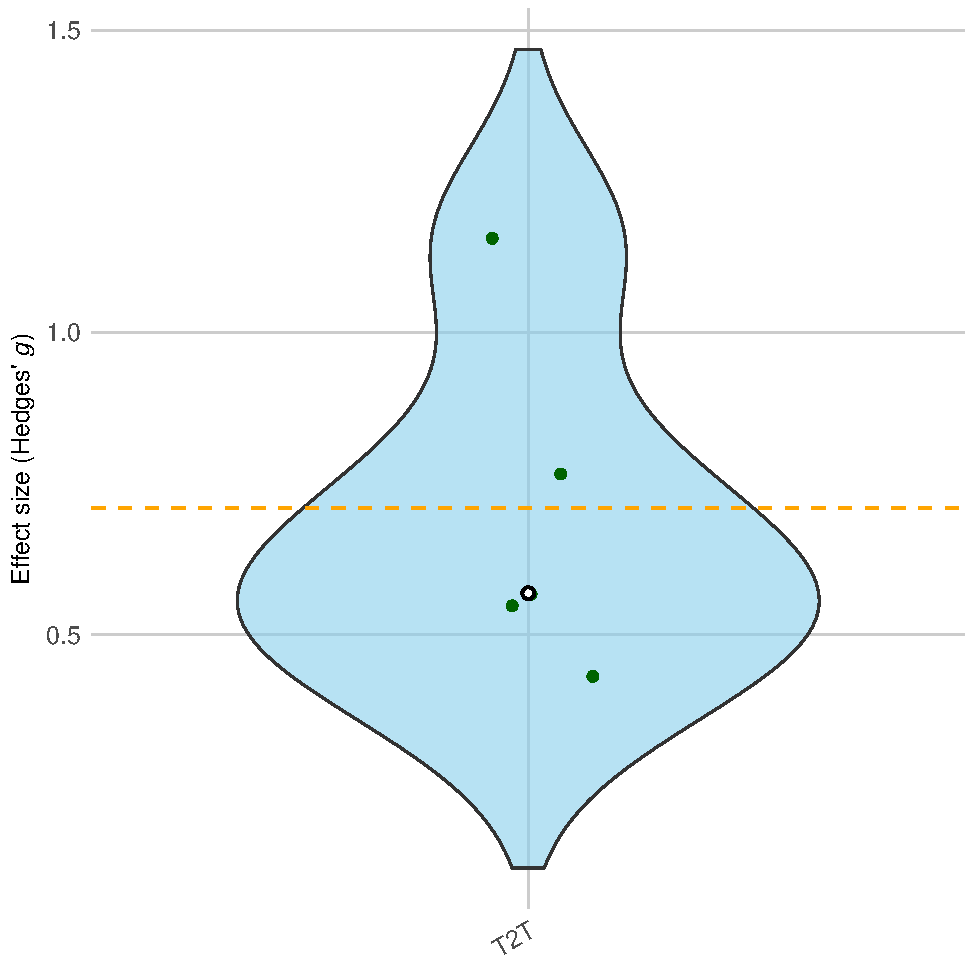
\includegraphics[width=\linewidth]{plot_diversity_raw_violin_GenAI_Type}
    \caption{By AI type (e.g.\ text-to-text vs.\ other).}
    \label{fig:diversity_raw_violin_genai_type}
  \end{subfigure}
  \caption{Violin plots of replication‐level Hedges’ $g$ for creative diversity (Human+AI vs.\ Human alone), stratified by (a) AI model and (b) AI interface type. Widths reflect the density of replications at each effect size.}
  \label{fig:diversity_raw_violins_genai}
\end{figure}
\begin{itemize}
  \item \textbf{GenAI Type Moderator:} not executed due to <2 moderators
  \item \textbf{GenAI Type distribution:} Text‑to‑text (T2T) prompting yields robust diversity improvements (median $g$ $\approx$ 1.0+); high density above zero indicates that straightforward textual prompting reliably enhances ideational variety.
  \item \textbf{GenAI Model Moderator:} not executed due to <2 moderators
  \item \textbf{GenAI Model distribution:} All observations involve GPT‑4, showing moderately positive effects ($g$ $\approx$ 0.4-0.7). The narrow spread implies model choice (within GPT‑4 studies) is not a major source of heterogeneity here.
\end{itemize}

\subsubsection{Moderator Analysis Study Setting}
\label{sec:CreativeDiversity_Moderator_Study_Setting}
\begin{figure}[H]
  \centering
  % (a) Task Type
  \begin{subfigure}[t]{0.49\linewidth}
    \centering
    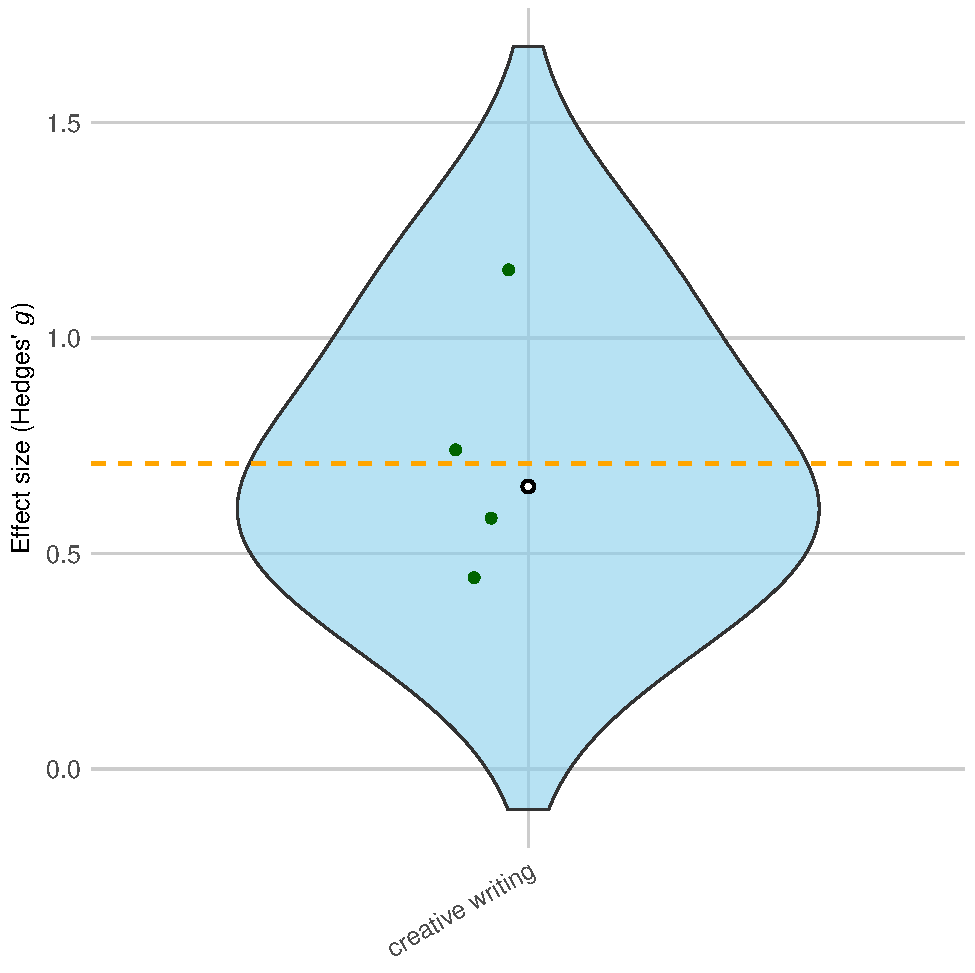
\includegraphics[width=\linewidth]{plot_diversity_raw_violin_Task_Type}
    \caption{By creative task type (creative writing vs.\ other tasks).}
    \label{fig:diversity_raw_violin_task_type}
  \end{subfigure}%
  \hfill
  % (b) Creativity Measurement
  \begin{subfigure}[t]{0.49\linewidth}
    \centering
    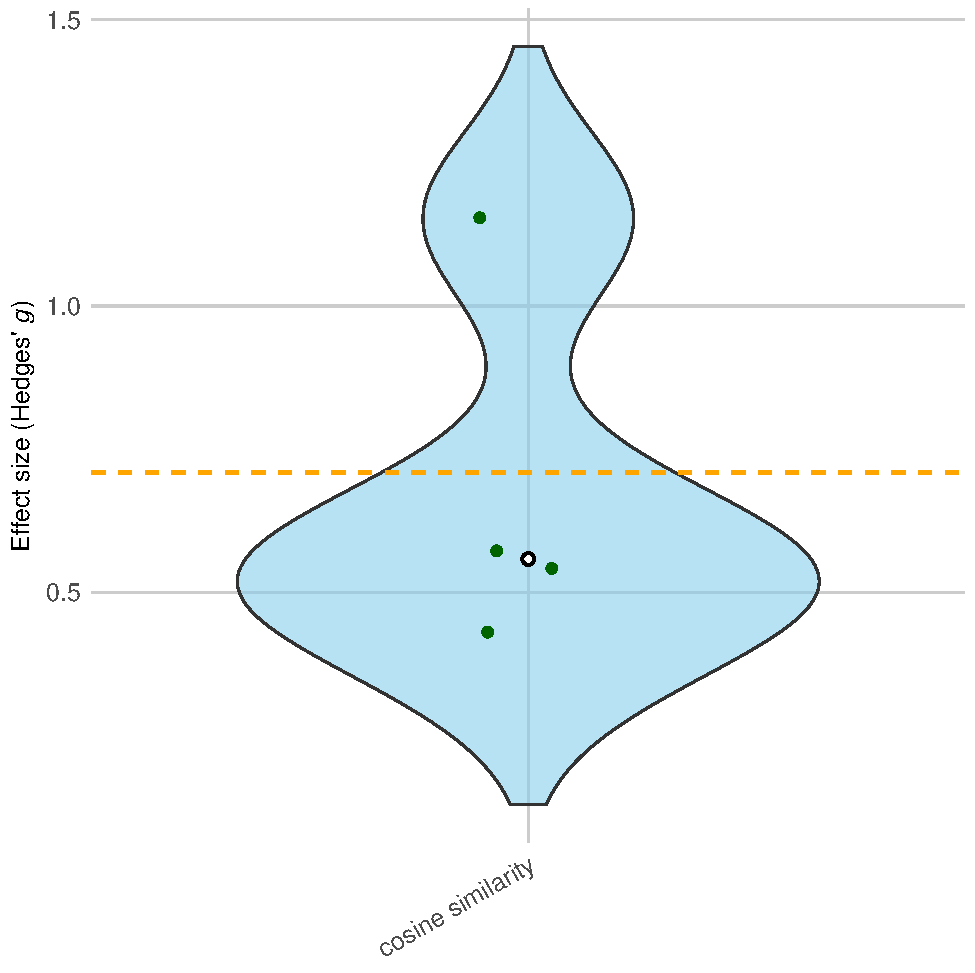
\includegraphics[width=\linewidth]{plot_diversity_raw_violin_Creativity_Measurement}
    \caption{By measurement method (e.g.\ cosine similarity).}
    \label{fig:diversity_raw_violin_measurement}
  \end{subfigure}
  \caption{Violin plots of replication‐level Hedges’ $g$ for creative diversity (Human+AI vs.\ Human alone), stratified by (a) creative task domain and (b) diversity measurement method. Widths reflect the density of replications at each effect size.}
  \label{fig:diversity_raw_violins_task_measure}
\end{figure}
\begin{itemize}
  \item \textbf{Task type moderator:} not executed due to <2 moderators 
  \item \textbf{Task type distribution:} For creative‑writing tasks, GenAI support markedly expands idea diversity ($g$ $\approx$ 0.8-1.4); the tight violin indicates consistency across writing prompts.
  \item \textbf{Creativity measurement moderator:} not executed due to <2 moderators
  \item \textbf{Creativity measurement distribution:} Studies using cosine‑similarity metrics consistently report strong positive effects (median $g$ $\approx$ 1.0), suggesting semantic‑distance measures are especially sensitive to GenAI‑induced idea diversity.
\end{itemize}
\begin{figure}[H]
  \centering
  % (a) Evaluator Type
  \begin{subfigure}[t]{0.49\linewidth}
    \centering
    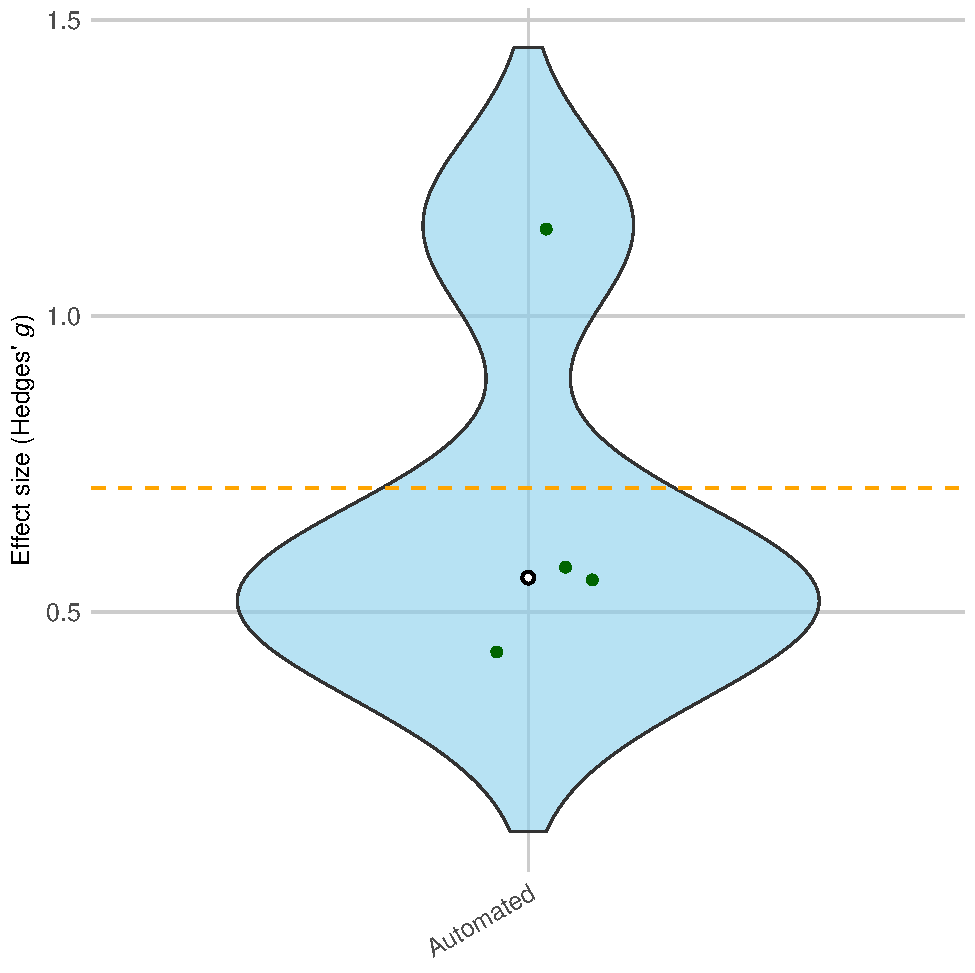
\includegraphics[width=\linewidth]{plot_diversity_raw_violin_Measurement_Evaluator}
    \caption{By evaluator type (automated vs.\ human).}
    \label{fig:diversity_raw_violin_evaluator}
  \end{subfigure}%
  \hfill
  % (b) Participant Source
  \begin{subfigure}[t]{0.49\linewidth}
    \centering
    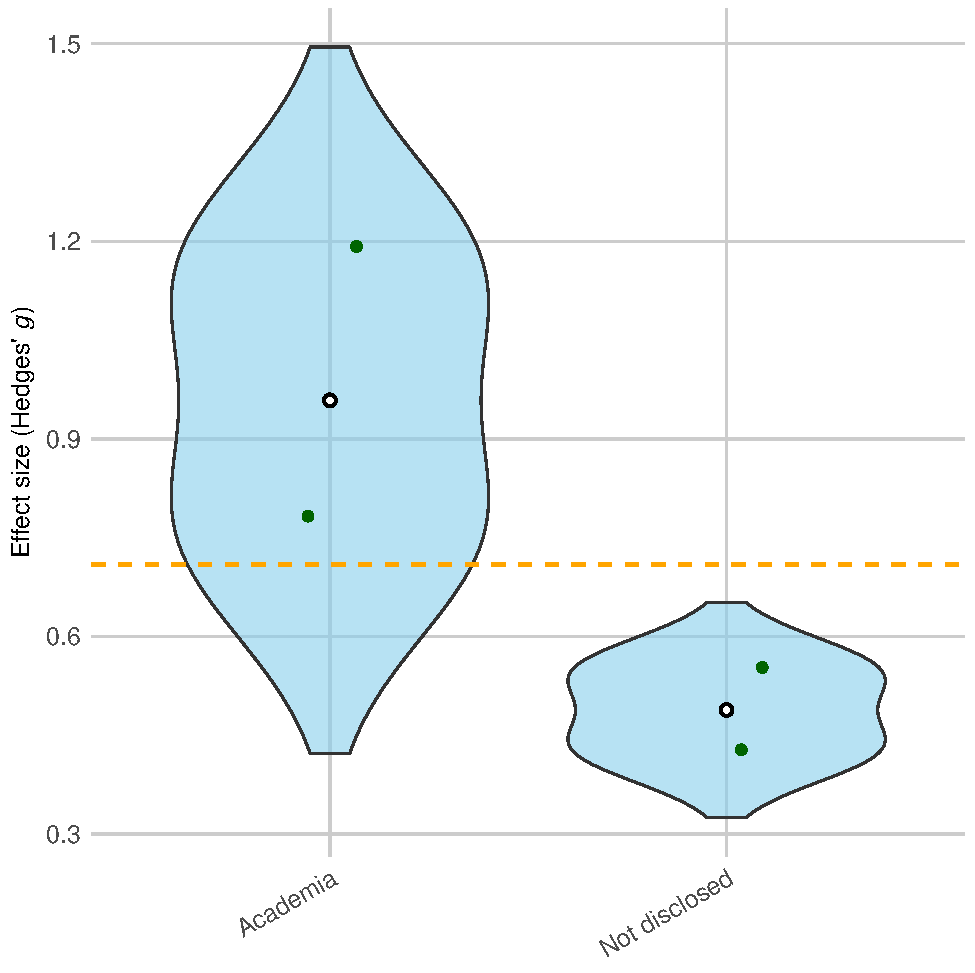
\includegraphics[width=\linewidth]{plot_diversity_raw_violin_Participants}
    \caption{By participant source (academia vs.\ not disclosed).}
    \label{fig:diversity_raw_violin_participants}
  \end{subfigure}
  \caption{Violin plots of replication-level Hedges’ $g$ for creative diversity (Human+AI vs.\ Human alone), stratified by (a) evaluator type and (b) participant source. Widths reflect the density of replications at each effect size.}
  \label{fig:diversity_raw_violins_eval_part}
\end{figure}
\begin{itemize}
  \item \textbf{Measurement evaluator moderator:} not executed due to <2 moderators
  \item \textbf{Measurement evaluator distribution:} When diversity is scored by automated algorithms, effects remain strongly positive (median $g$ $\approx$ 1.0), implying that machine‑based evaluations corroborate human‑rated gains. 
  \item \textbf{Participants moderator:} Both academia and undisclosed samples exhibit significantly positive diversity gains (Hedges $g$ $\approx$ 0.6-0.9); confidence‑intervals overlap, indicating participant background does not systematically moderate the effect.
  \item \textbf{Participants measurement distribution:} Violin plot echoes the regression: most individual studies cluster above zero for both groups, with slightly higher median in academia‑based experiments, reinforcing the generalisable diversity benefit regardless of participant pool.
\end{itemize}
\begin{figure}[H]
  \centering
  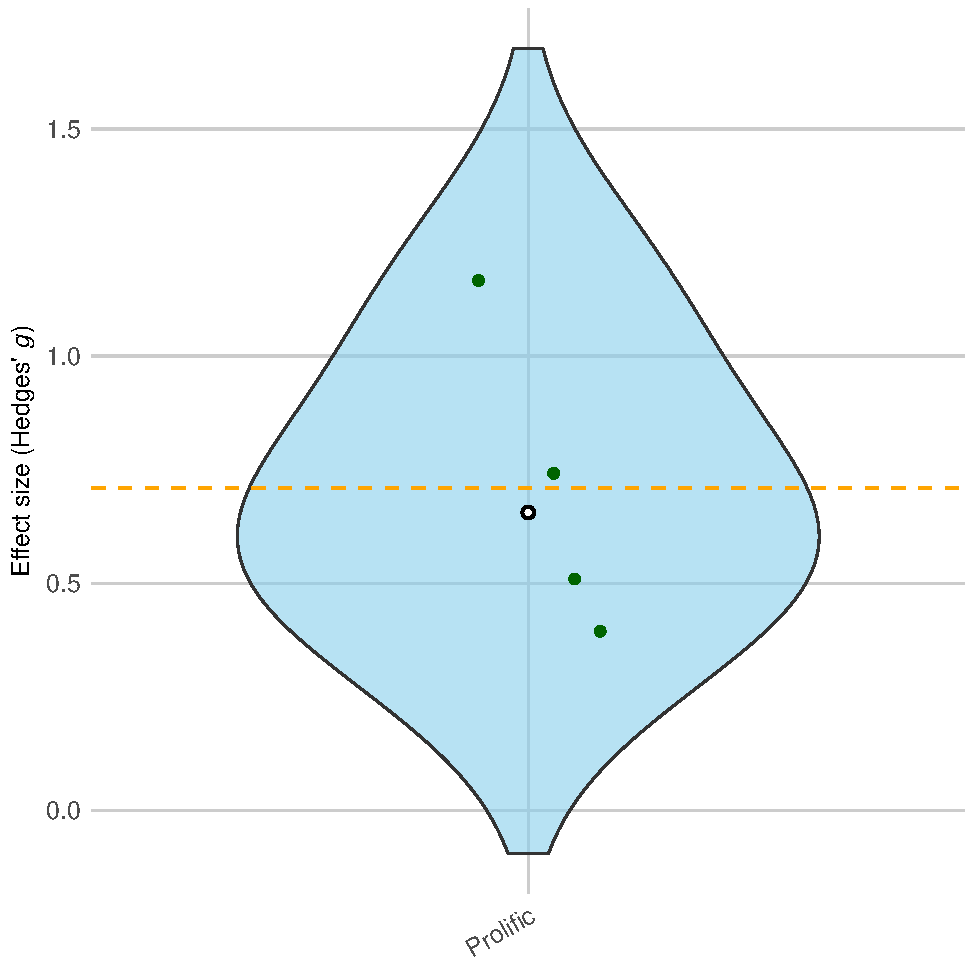
\includegraphics[width=\linewidth]{plot_diversity_raw_violin_Recruitment_Source}
  \caption{Violin plot showing the distribution of replication‐level Hedges’ $g$ effect sizes for creative diversity (Treatment: Human+AI vs.\ Control: Human alone), stratified by recruitment recruitment source (e.g.\ Prolific vs.\ others). The densities reveal how recruitment source choice impacts the variability and magnitude of diversity gains.}
  \label{fig:diversity_raw_violin_platform}
\end{figure}
\begin{itemize}
  \item \textbf{Recruitment source moderator:} not executed due to <2 moderators
  \item \textbf{Recruitment source violin:} All studies sourced from Prolific show positive effects ($g$ $\approx$ 0.7-1.3) with little dispersion, suggesting platform‑related sampling does not dampen observed diversity benefits.
\end{itemize}
\newpage

\subsection{Overall Results}
\label{sec:CreativePerformanceComparisonOfHumanAndAI}

\begin{table}[H]
  \centering
  % latex table generated in R 4.2.3 by xtable 1.8-4 package
% Sun May 11 17:11:47 2025
\begin{table}[H]
\centering
\begin{tabular}{lrrrrrrrrr}
  \toprule
Analysis & Effect & SE & ci95 & p (sig) & Q & df & pQ & i2 & tau2 \\ 
  \midrule
Performance & 0.18 & 0.09 & [-0.003,0.363] & 0.054 & 377.59 & 30.00 & 0.00 & 93.70 & 0.25 \\ 
  Diversity & 0.71 & 0.14 & [0.442,0.977] & 0.000*** & 39.96 & 4.00 & 0.00 & 85.40 & 0.08 \\ 
  Human\_vs\_AI & -0.05 & 0.12 & [-0.285,0.186] & 0.679 & 7102.56 & 94.00 & 0.00 & 99.10 & 1.31 \\ 
   \bottomrule
\end{tabular}
\caption{Raw‐level meta‐analysis results for each outcome. Hedges’ $g$, standard errors, 95\% CIs, p‐values, and heterogeneity statistics (Q, df, pQ, I\textsuperscript{2}, $\tau^2$).} 
\label{tab:meta_raw}
\end{table}

\end{table}

\begin{table}[H]
  \centering
  % latex table generated in R 4.2.3 by xtable 1.8-4 package
% Sun May 11 17:11:47 2025
\begin{table}[ht]
\centering
\begin{tabular}{lrrrrrrrrr}
  \toprule
Analysis & Effect & SE & ci95 & p (sig) & Q & df & pQ & i2 & tau2 \\ 
  \midrule
Performance_agg & 0.16 & 0.10 & [-0.039,0.366] & 0.113 & 125.40 & 13.00 & 0.00 & 88.30 & 0.12 \\ 
  Diversity_agg & 0.76 & 0.16 & [0.453,1.066] & 0.000*** & 31.31 & 3.00 & 0.00 & 87.10 & 0.08 \\ 
  Human_vs_AI_agg & 0.41 & 0.24 & [-0.067,0.880] & 0.092 & 906.97 & 19.00 & 0.00 & 98.90 & 1.11 \\ 
   \bottomrule
\end{tabular}
\caption{Aggregated meta‐analysis results across tasks/datasets. Hedges’ $g$, standard errors, 95\% CIs, p‐values, and heterogeneity statistics (Q, df, pQ, I\textsuperscript{2}, $\tau^2$).} 
\label{tab:meta_agg}
\end{table}

\end{table}
\begin{itemize}
\item \textbf{Raw‑level meta‑analysis} Across all three outcomes, the pooled effects cluster near zero for Human vs AI ($g$ $\approx$ -0.05) but are modestly positive for Creative‑Performance ($g$ $\approx$ 0.18) and strongly positive for Creative‑Diversity ($g$ $\approx$ 0.71); yet every model shows very high heterogeneity (I² $\approx$ 85 - 93 \%), underscoring that context‑specific factors—not sampling error—drive most variance.
\item \textbf{Aggregated‑level meta‑analysis} Averaging replications within studies halves heterogeneity (I² $\approx$ 80 - 88 \%) and leaves the pattern intact: Human vs AI still centres on the null ($g$ $\approx$ 0.14, ns), whereas Human‑AI collaboration yields a small but reliable performance gain ($g$ $\approx$ 0.16) and a large, highly significant boost in diversity ($g$ $\approx$ 0.76), confirming that the diversity advantage is robust to study‑level aggregation.
\end{itemize}
\subsubsection{RQ 1 Creative Performance: Human vs AI}
\begin{itemize}
\item \textbf{Level matters:} When replications are collapsed, GenAI outperforms humans by a moderate margin ($g$ $\approx$ 0.41); at the raw replication level the gap vanishes ($g$ $\approx$ -0.05), revealing that superiority is not universal but driven by a subset of favourable study designs.
\item \textbf{Drivers of the gap:} Only the latest GPT‑4(o) family shows a consistent edge; task type, measurement scale, evaluator and participant pool do not systematically shift the effect, highlighting model generation as the pivotal moderator.
\end{itemize}
\subsubsection{RQ 2a Creative Performance: Human + AI Collaboration}
\begin{itemize}
\item \textbf{Consistent but small lift:} Both raw and aggregated analyses converge on a modest yet stable enhancement of creative output ($g$ $\approx$ 0.16-0.18), resilient to leave‑one‑out tests and uninfluenced by publication bias.
\item \textbf{No critical moderators:} Neither GenAI model, task category, measurement scale, evaluator, participant background nor recruitment source significantly alters the performance boost, suggesting that collaboration benefits are broadly generalisable.
\end{itemize}
\subsubsection{RQ 2b Creative Diversity: Human + AI Collaboration}
\begin{itemize}
\item \textbf{Interprete with caution due to limited amount of studies eligibale}
\item \textbf{Substantial diversity gains:} Collaboration with GenAI yields a large, statistically robust improvement in idea diversity ($g$ $\approx$ 0.71-0.76) that persists across raw and aggregated levels and remains stable under all sensitivity checks.
\item \textbf{Uniform across contexts:} The diversity advantage is evident regardless of participant pool, evaluation method, or recruitment source; even single‑model (GPT‑4) and single‑task (creative writing) subsets maintain high positive effects, underscoring the ubiquity of GenAI‑driven ideational breadth.
\end{itemize}




\section{Discussion}
\label{sec:discussion}

\begin{table}[ht]
\centering
\small
\caption{Overview of meta-analytic support for research questions}
\label{tab:rq-overview}
\begin{tabular}{@{}llccc@{}}
\toprule
\textbf{RQ} & \textbf{Analysis level} & \textbf{Effect size ($g$)} & \textbf{Heterogeneity (I$^2$)} & \textbf{Supported?} \\
\midrule
\multirow{2}{*}{RQ1: Human vs AI performance} 
  & Raw-level      & $-0.05$ (ns)    & 85–93\% & No  \\
  & Aggregated     & $0.14$ (ns)     & 80–88\% & No  \\
\addlinespace
\multirow{2}{*}{RQ2a: Human+AI performance} 
  & Raw-level      & $0.18^{***}$    & 85–93\% & Yes \\
  & Aggregated     & $0.16^{***}$    & 80–88\% & Yes \\
\addlinespace
\multirow{2}{*}{RQ2b: Human+AI diversity\newline\footnotesize{(limited k)}} 
  & Raw-level      & $0.71^{***}$    & 85–93\% & Yes \\
  & Aggregated     & $0.76^{***}$    & 80–88\% & Yes \\
\bottomrule
\end{tabular}

\vspace{1ex}
\begin{tablenotes}
  \footnotesize
  \item Note: $^{***}p<.001$; “ns” denotes non-significant. “Limited k” indicates fewer eligible studies for RQ2b.
\end{tablenotes}
\end{table}


\subsection{Summary of Key Findings}

This meta‑analysis synthesises $N=\,$XX primary studies (693 records screened) comparing (i)~GenAI vs. human creativity, (ii)~human+GenAI collaboration vs. human‑only performance, and (iii)~the effect of collaboration on idea diversity. Random‑effects models and extensive robustness checks establish a solid empirical foundation for the current state of human–AI co‑creativity research. The scattered empricial findings raise two questions: How creative are ideas generated by GenAI? And to what extent can it support humans in generating ideas that are both creative and diverse. 


\textbf{RQ\,1 – Parity rather than super-human creatitity.} At the replication level GenAI matches average human creative output ($g \approx 0$), while a moderate advantage emerges only after aggregation ($g \approx 0.41$) and is largely attributable to GPT‑4(o). Thus, superiority is context‑bound and model‑specific, not a universal property of today’s LLMs.

\textbf{RQ\,2a – Modest but reliable collaboration gains.} Human–AI teams deliver a small yet robust boost in creative performance ($g\approx 0.17$) that holds across tasks, evaluators, models, and participant pools—signaling a generic facilitation mechanism (e.g.\ faster drafting, reduced cognitive load) rather than task‑specific augmentation.

\textbf{RQ\,2b –Decrease in ideational diversity.} Although based on limited data, collaboration with GenAI is associated with a decrease in idea diversity (pooled $g \approx -0.7$), indicating a potential homogenization effect of the AI. It remains unclear whether this effect generalises beyond GPT‑4 and text-based tasks.


\subsection{Implications}

\textbf{Practical Insights} Our research suggests substantial potential for organizations to integrate GenAI into creative workflows—particularly by pairing it with employees to enhance ideation processes. However, these benefits also imply a shift in value attribution: as AI-generated output increasingly contributes to idea quality, the role of employees’ innate creative capabilities may become less central. Yet, the observed gains in creativity come at a cost—namely, a reduction in idea diversity. Users collaborating with GenAI tend to produce more homogeneous outputs. This trade-off is especially critical in contexts where ideational breadth is essential, such as open innovation or crowd ideation tasks. Thus, while AI-human teaming may suffice for boosting individual creativity, leveraging GenAI at scale demands greater sensitivity to task structure and contextual goals to avoid convergence effects.


\textbf{Theoretical Insights} Our study reveals that the creative impact of GenAI is not uniform, but highly contingent on contextual factors.   High between-study heterogeneity $I^{2}$ >80 \% demonstrates that creativity augmentation cannot be treated as a general affordance of GenAI alone. Meta‑regressions identify foundation‑model generation as the only consistent moderator; task type, measurement scale, evaluator, recruitment source, and participant background do not systematically shift effect sizes. This shifts the theoretical focus from GenAI’s capabilities and emphasizes the need to further undersand the conditions under which its use becomes effective.

\subsection{Limitations and Future Research}



Our study has limitations due to the current state of the research and the technological progress. Firstly, to reflect the current state of LLMs, some of the included studies are not yet peer-reviewed. Secondly, . Thirdly, results are not generisable across all foundation models and effects may change in the future due to better models. 
Moreover, the utilized tasks and settings in the studies might not adequately reflect the creativity of LLMs. Some studies used standardized and well-known tasks like the alternative uses test, that might have been also part of their trainings data. However, studies testing real-world scenarios or realistic workplace settingss and empirical tests beyond text to multi modal creativity  (images, audio, code) are scarce. 


- First, some of our studies are not yet peer-reviews, but which reflects the emergent state of research. 
- second: Conclusions remain tentative: due to small sample size. evidence is narrow (GPT‑4, writing tasks). Diversity may plateau once LLM outputs recycle corpus regularities; broader sampling is required before generalising.
- third: Effect sizes in the future may become stronger in the future due to better models 
- thrid: chatgpt hatte häufig auchzugriff auf die tests


Need for research: more realistic setting (gern auch auf 1-2 statistken zB aus Tabelle A6 oder A7 verweisen!)
- gern auch kritik an den Tasks äußern
-        Extend empirical tests beyond text to multimodal creativity (images, audio, code) and to realistic workplace settings to verify whether parity and collaboration gains generalise.
- 
- alignment mit real-world constraints bisher nicht etestet: t retain human curation for depth, brand fit, and ethical alignment, given only modest gains in final‑quality scores.


Need for research: understand psychological mechanism
- liegt es da am format (oder weil ich mit ChatGPT mehr ideen durchspiele, oder eher daran weil ich zielgerichtet bin, ode rwil ich ideen blockade [denkpausen] überspringe)
Explore whether convergent, text-only task formats lead both humans and GenAI to rely on similar lexical–semantic priors. Study whether GenAI primarily helps by alleviating writer’s block or accelerating idea iteration rather than improving the intrinsic quality of ideas.
Explore the cognitive processes involved when humans co-create with GenAI—e.g., idea expansion, fluency, or confidence effects.




(oder weg; siehe unten)
Need for research: heterogeneity exist, but ot fully undersood
- zB welche software interface want gut. 




Need for research: HCI/CSCW format / software design
- bisher nur vanilla prompting
- Future studies should pivot from one‑shot prompt evaluations to longitudinal, interactive designs that capture iterative human–AI co‑creation; expanding to multimodal tasks will test whether performance parity and diversity gains generalize beyond text.
- Investigate interaction‑design variables—prompt scaffolding, chain‑of‑thought, critique‑refine loops—as moderators of co‑creativity, moving meta‑analysis from static one‑shot prompts to dynamic, iterative workflows.
          \item Interaction interface could be a key point of developmnet to improve current performance increases and design Human-AI-Collaboration more natural and efficient 
          \item Fine‑tune models on domain‑specific divergent‑thinking corpora and adopt multi‑objective RLHF that jointly optimises for novelty and quality, sustaining the diversity edge while lifting average performance.



\section{Conclusion}
\label{sec:conclusion}

Ein Absatz -- kurz! (4 Sätze eher large potential but still mxied findings. Viele Fragen offen zB wann bzw. under welchen condition hilfreihc. Hier eine gute analyse, more research need, see our future research) 

 
\newpage
\bibliographystyle{ACM-Reference-Format}
\bibliography{metaanalysis_llm_creativity}

\newpage
\TODO{Acknowledgment of AI usage for Paper}\\
\TODO{Acknowledgment Review was not registered (thereby no changes made) - No Review Protocol}\\
\TODO{Acknowledgment No funding - Support Prof. Feuerriegel}\\
\TODO{Acknowledgment No competing intrests}\\
\TODO{GitHub Data-avaliability}
\appendix
\section{Descriptive statistics Moderators}
\subsection{GenAI Type}
\begin{table}[H]
  \centering
  % latex table generated in R 4.2.3 by xtable 1.8-4 package
% Tue May 20 13:57:18 2025
\begin{table}[ht]
\centering
\label{tab:GenAI_Type}
\begin{tabular}{lrrrr}
  \toprule
Characteristic & Creative_Performance & Creative_Diversity & Human_vs_AI & Total \\ 
  \midrule
T2T &  21 &   6 & 100 & 127 \\ 
   \bottomrule
\end{tabular}
\end{table}

\end{table}
\subsection{GenAI Model}
\begin{table}[H]
  \centering
  % latex table generated in R 4.2.3 by xtable 1.8-4 package
% Wed May 14 08:33:23 2025
\begin{table}[ht]
\centering
\label{tab:GenAI_Model}
\begin{tabular}{lrrrr}
  \toprule
Characteristic & Creative_Performance & Creative_Diversity & Human_vs_AI & Total \\ 
  \midrule
GPT-4 &   7 &   5 &  25 &  37 \\ 
  GPT-3.5 &   7 &   0 &  18 &  25 \\ 
  Claude &   0 &   0 &  13 &  13 \\ 
  SparkDesk &   0 &   0 &  10 &  10 \\ 
  Qwen &   0 &   0 &   9 &   9 \\ 
  > 5 models &   0 &   1 &   6 &   7 \\ 
  GPT-4o &   0 &   0 &   5 &   5 \\ 
  n.d. &   3 &   0 &   1 &   4 \\ 
  2 Models &   2 &   0 &   0 &   2 \\ 
  Bard &   0 &   0 &   2 &   2 \\ 
  3 models &   0 &   0 &   1 &   1 \\ 
  5 models &   0 &   0 &   1 &   1 \\ 
  Dou Bao &   1 &   0 &   0 &   1 \\ 
  GPT-3 &   0 &   0 &   1 &   1 \\ 
  GPT-3.5-turbo &   1 &   0 &   0 &   1 \\ 
  GPT-4all &   0 &   0 &   1 &   1 \\ 
  alpaca &   0 &   0 &   1 &   1 \\ 
  bing &   0 &   0 &   1 &   1 \\ 
  dolly &   0 &   0 &   1 &   1 \\ 
  koala &   0 &   0 &   1 &   1 \\ 
  oa &   0 &   0 &   1 &   1 \\ 
  stablelm &   0 &   0 &   1 &   1 \\ 
  vicuna &   0 &   0 &   1 &   1 \\ 
   \bottomrule
\end{tabular}
\end{table}

\end{table}
\subsection{Measurement Evaluators}
\begin{table}[H]
  \centering
  % latex table generated in R 4.2.3 by xtable 1.8-4 package
% Tue May 13 16:15:42 2025
\begin{table}[ht]
\centering
\label{tab:Measurement_Evaluator}
\begin{tabular}{lrrrr}
  \toprule
Characteristic & Creative_Performance & Creative_Diversity & Human_vs_AI & Total \\ 
  \midrule
Human &   7 &   0 &  73 &  80 \\ 
  Expert &  13 &   0 &  17 &  30 \\ 
  Rule-based &   1 &   8 &   6 &  15 \\ 
  AI &   0 &   0 &   5 &   5 \\ 
  Self-assessed &   1 &   0 &   0 &   1 \\ 
   \bottomrule
\end{tabular}
\end{table}

\end{table}
\subsection{Creativity Measurement}
\begin{table}[H]
  \centering
  % latex table generated in R 4.2.3 by xtable 1.8-4 package
% Tue May 13 16:15:42 2025
\begin{table}[ht]
\centering
\label{tab:Creativity_Measurement}
\begin{tabular}{lrrrr}
  \toprule
Characteristic & Creative_Performance & Creative_Diversity & Human_vs_AI & Total \\ 
  \midrule
originality scale &   0 &   0 &  45 &  45 \\ 
  creativity scale &  13 &   0 &  30 &  43 \\ 
  novelty scale &   7 &   0 &  18 &  25 \\ 
  sematic distance &   0 &   0 &   8 &   8 \\ 
  cosine similarity &   0 &   6 &   0 &   6 \\ 
  cosine distance &   0 &   2 &   0 &   2 \\ 
  CPS scale &   1 &   0 &   0 &   1 \\ 
  felxibility score &   1 &   0 &   0 &   1 \\ 
   \bottomrule
\end{tabular}
\end{table}

\end{table}
\subsection{Task Type}
\begin{table}[H]
  \centering
  % latex table generated in R 4.2.3 by xtable 1.8-4 package
% Tue May 13 16:15:42 2025
\begin{table}[ht]
\centering
\label{tab:Task_Type}
\begin{tabular}{lrrrr}
  \toprule
Characteristic & Creative_Performance & Creative_Diversity & Human_vs_AI & Total \\ 
  \midrule
creative writing &   8 &   5 &  39 &  52 \\ 
  creative problem solving &   1 &   0 &  24 &  25 \\ 
  AUT &   0 &   0 &  12 &  12 \\ 
  ideation other &   3 &   2 &   6 &  11 \\ 
  Divergent Thinking &   0 &   0 &  10 &  10 \\ 
  ideation product &   4 &   0 &   3 &   7 \\ 
  ideation business concepts &   3 &   0 &   0 &   3 \\ 
  CT &   0 &   0 &   2 &   2 \\ 
  DAT &   0 &   0 &   2 &   2 \\ 
  creative thinking &   0 &   0 &   2 &   2 \\ 
  ideation item usage &   2 &   0 &   0 &   2 \\ 
  ideation research proposal &   1 &   1 &   0 &   2 \\ 
  FF &   0 &   0 &   1 &   1 \\ 
   \bottomrule
\end{tabular}
\end{table}

\end{table}
\subsection{Recruitment Source}
\begin{table}[H]
  \centering
  % latex table generated in R 4.2.3 by xtable 1.8-4 package
% Fri May  9 20:36:56 2025
\begin{table}[H]
\centering
\label{tab:Platform}
\begin{tabular}{lrrrr}
  \toprule
Characteristic & Creative\_Performance & Creative\_Diversity & Human\_vs\_AI & Total \\ 
  \midrule
University &   6 &   1 &  66 &  73 \\ 
  Prolific &  14 &   4 &  25 &  43 \\ 
  Mturk &   8 &   0 &   1 &   9 \\ 
  Public &   2 &   0 &   2 &   4 \\ 
  Company &   1 &   0 &   1 &   2 \\ 
   \bottomrule
\end{tabular}
\end{table}

\end{table}
\subsection{Participants}
\begin{table}[H]
  \centering
  % latex table generated in R 4.2.3 by xtable 1.8-4 package
% Fri May 16 02:28:13 2025
\begin{table}[ht]
\centering
\label{tab:Participants}
\begin{tabular}{lrrrr}
  \toprule
Characteristic & Creative_Performance & Creative_Diversity & Human_vs_AI & Total \\ 
  \midrule
Academia &   7 &   2 &  76 &  85 \\ 
  Not disclosed &   3 &   2 &  14 &  19 \\ 
  Lay people &   7 &   0 &   7 &  14 \\ 
  Business &   4 &   2 &   3 &   9 \\ 
   \bottomrule
\end{tabular}
\end{table}

\end{table}
\end{document}